%!TEX root = ../thesis.tex
%*******************************************************************************
%*********************************** Fourth Chapter *****************************
%*******************************************************************************


\chapter{Results and analysis}  %Title of the Fourth Chapter

\ifpdf
     \graphicspath{{Figs/Chapter4/}}
\else
    \graphicspath{{Chapter4/Figs/Vector/}{Chapter4/Figs/}}
\fi

This chapter examines the three hypotheses of this study, including the application of training algorithm optimisations to recursive neural tensor networks (NTNs), compensating for covariate shift introduced by hypernetworks during convolutional tensor factorisation, and finally the initialisation of entity and relation embeddings using pre-trained word vectors. 


%********************************** %Recursive Neural Tensor Networks  **************************************

\section{Recursive neural tensor networks}

\subsection{Datasets} 

For the first set of experiments we use the WordNet \unskip ~\citep{miller1995wordnet} and Freebase \unskip ~\citep{bollacker2008freebase} link prediction benchmark datasets.\ WordNet is a lexical database for English, and a taxonomy with hypernym relationships ("is a") and synonym sets. Freebase is a large collaborative knowledge base consisting of data about the world, composed mainly by community members. It is an online collection of structured data harvested from many sources, including user-submitted wiki contributions. The WordNet dataset contains a total of 136,611 triples, and Freebase a total of 375,499 triples. Visualisations of the respective knowledge graphs (KGs), as well as a sample of resource description framework (RDF) triple encoded facts, are presented in Figures 4.1 to 4.4. KG summary statistics are presented in Figures 4.5 to 4.7, and Table 4.1.

\begin{figure}
   	\centering
    	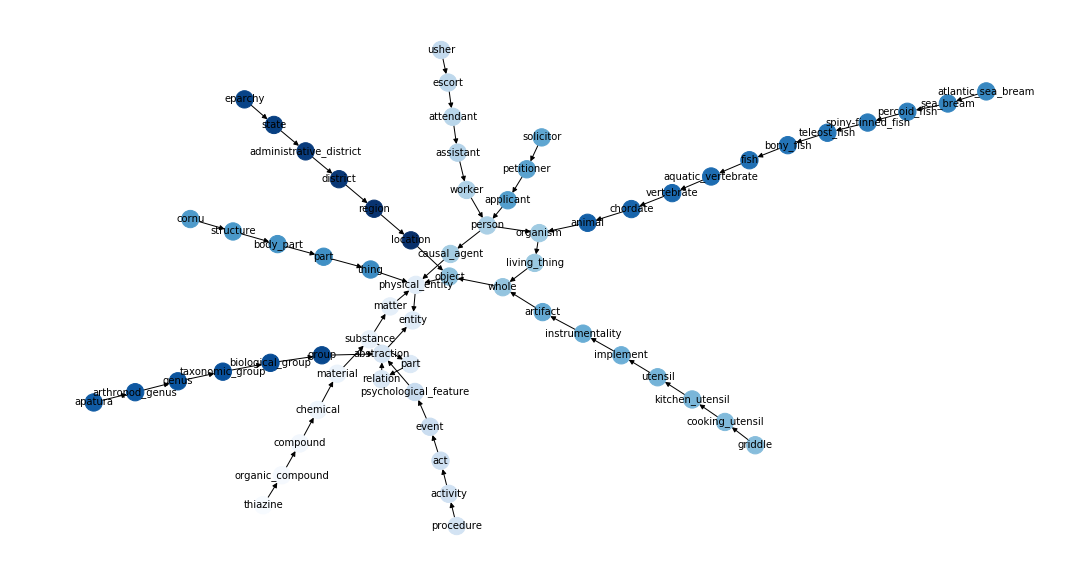
\includegraphics[width=0.9\textwidth, height=0.5\textwidth]{Wordnet}
	\captionsetup{justification=centering}
	\caption{A subset of WordNet facts structured as a KG. Entities are nodes, and relations are edges, where facts are encoded as RDF triples.}
\end{figure}

\begin{figure}
   	\centering
    	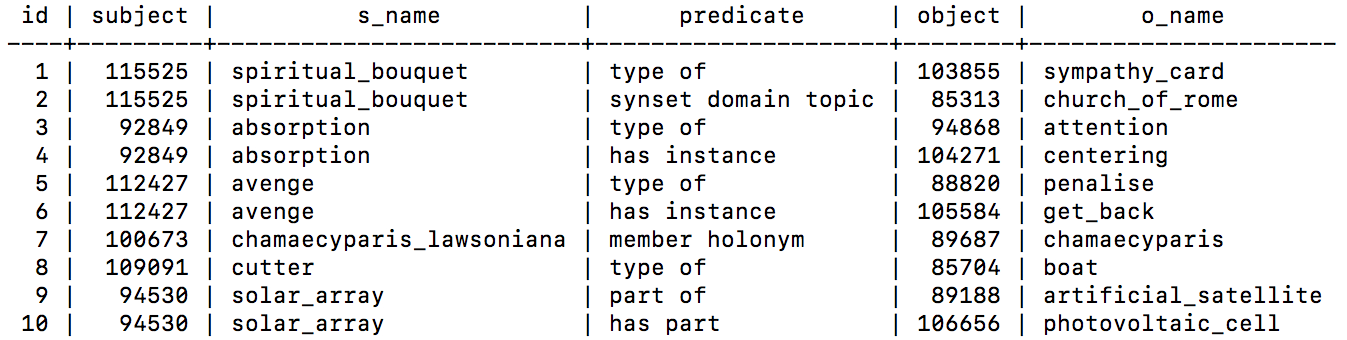
\includegraphics[width=0.9\textwidth, height=0.2\textwidth]{wordnet_fact_sample}
	\captionsetup{justification=centering}
	\caption{A sample of RDF triples from the WordNet KG.}
\end{figure}

\begin{figure}
   	\centering
    	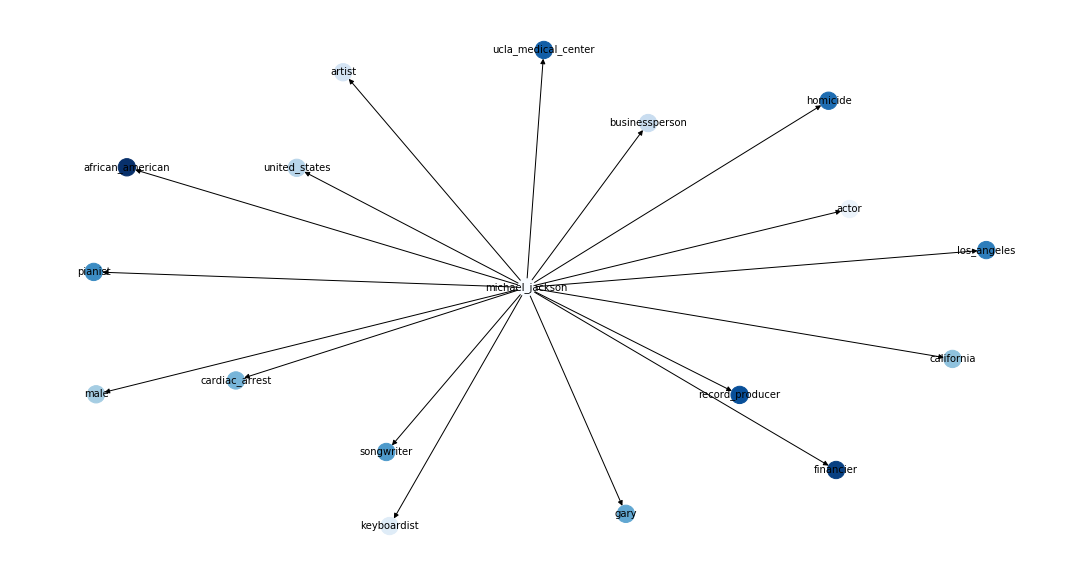
\includegraphics[width=0.9\textwidth, height=0.5\textwidth]{Freebase}
	\captionsetup{justification=centering}
	\caption{A subset of Freebase facts structured as a KG. Due to the size of Freebase, only a subset of facts related to the subject "Michael Jackson" is presented.}
\end{figure}

\begin{figure}
   	\centering
    	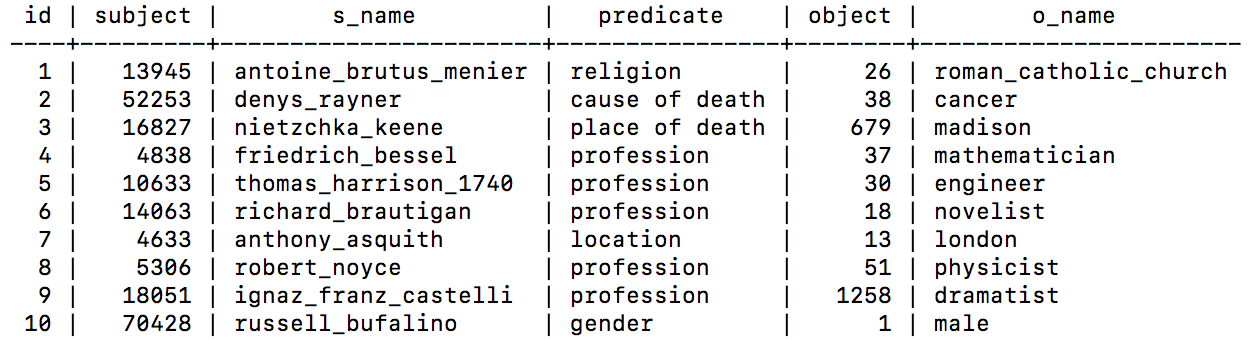
\includegraphics[width=0.9\textwidth, height=0.2\textwidth]{freebase_fact_sample}
	\captionsetup{justification=centering}
	\caption{A sample of RDF triples from the Freebase KG.}
\end{figure}


%********************************** %Subject **************************************

\begin{figure}
	\begin{subfigure}[b]{.5\linewidth}
   		\centering
    		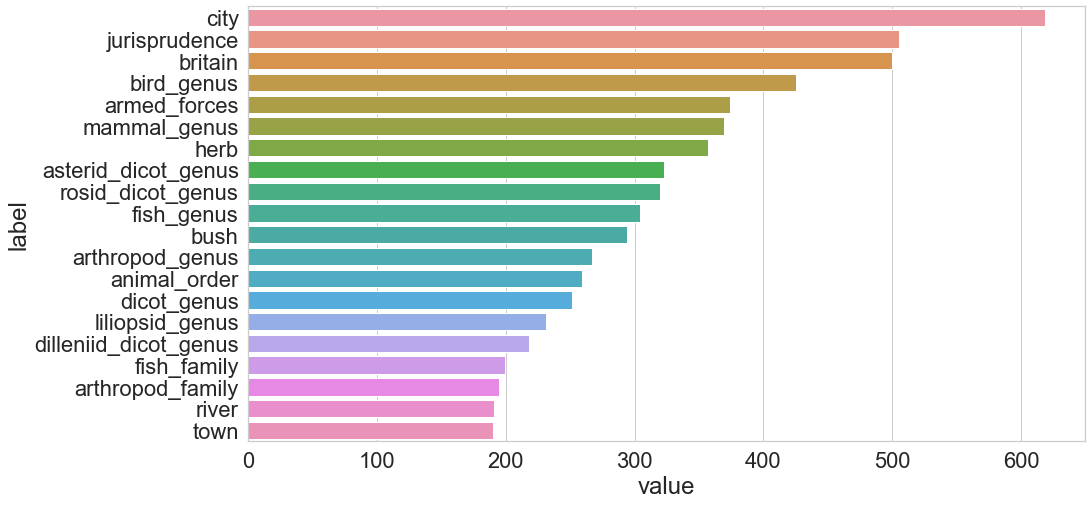
\includegraphics[width=1.0\linewidth, height=0.6\linewidth]{Wordnet_Subject_Counts}
		\captionsetup{justification=centering}
		\caption{WordNet}
	\end{subfigure}
	\begin{subfigure}[b]{.5\linewidth}
   		\centering
		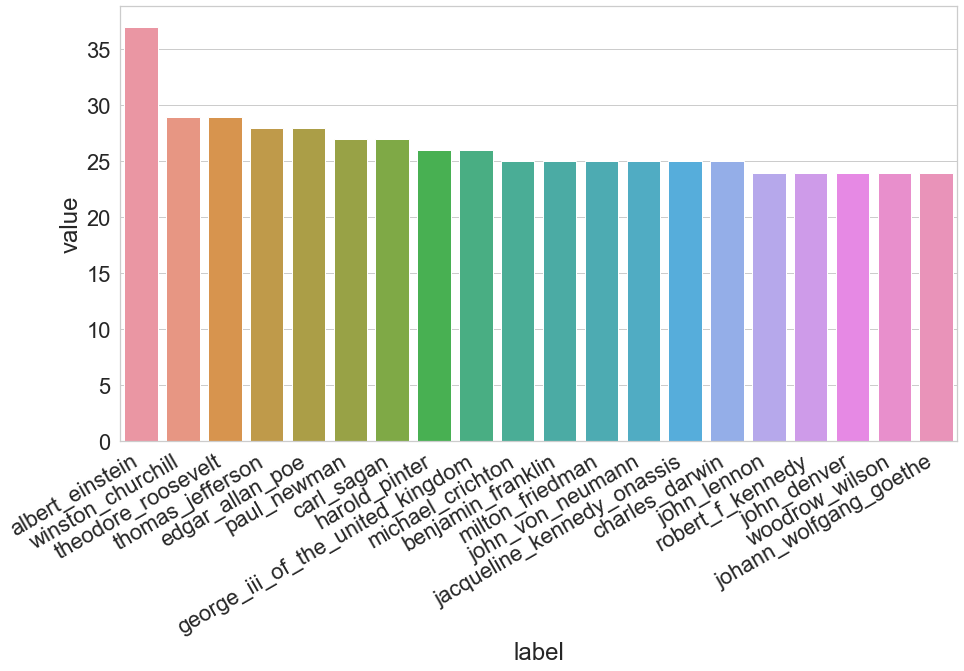
\includegraphics[width=1.0\linewidth, height=0.6\linewidth]{Freebase_Subject_Counts}
		\captionsetup{justification=centering}
		\caption{Freebase}
	\end{subfigure}
	\captionsetup{justification=centering}
	\caption{Histogram showing the number of times the 20 most frequent subject labels occur in KG facts, in the WordNet and Freebase link prediction datasets.}
\end{figure}


%********************************** %Predicate  **************************************


\begin{figure}
	\begin{subfigure}[b]{.5\linewidth}
   		\centering
    		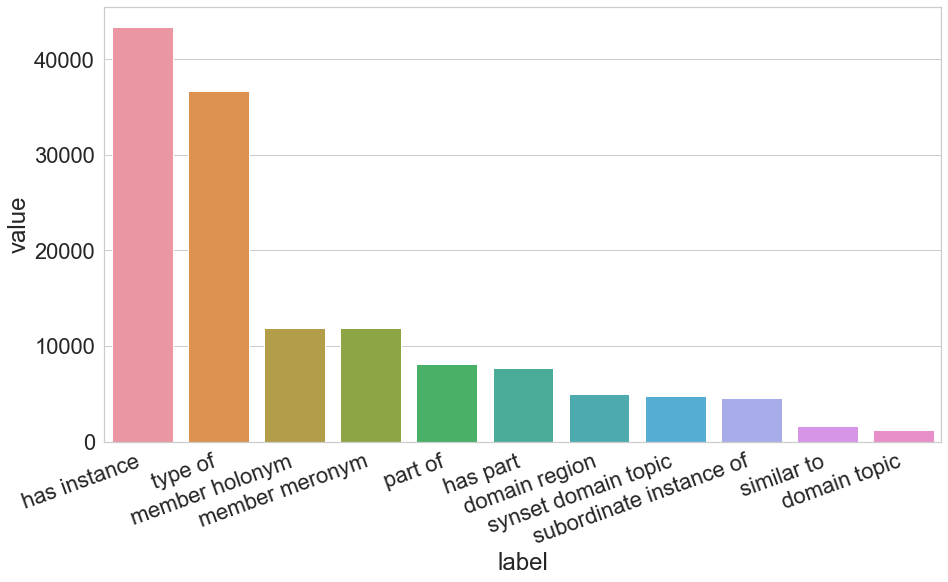
\includegraphics[width=1.0\linewidth, height=0.6\linewidth]{Wordnet_Predicate_Counts}
		\captionsetup{justification=centering}
		\caption{WordNet}
	\end{subfigure}
	\begin{subfigure}[b]{.5\linewidth}
   		\centering
		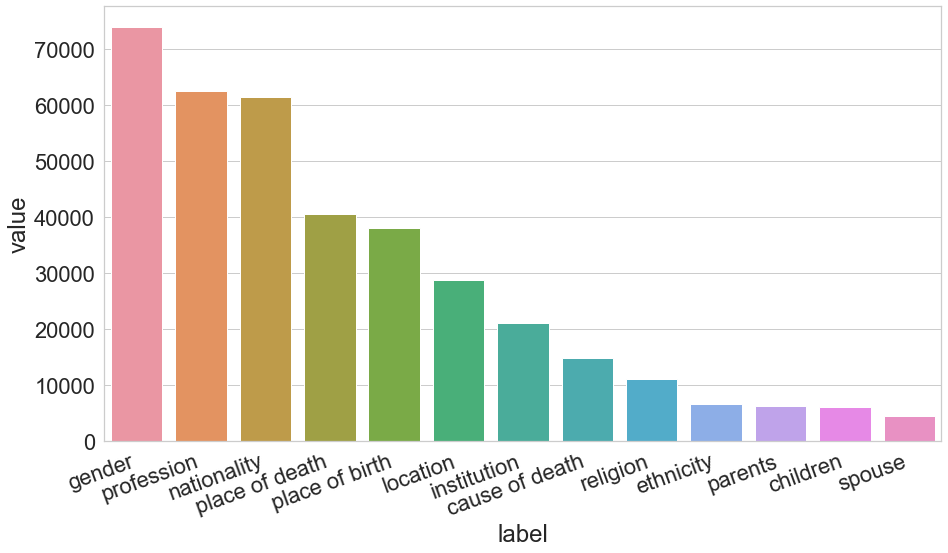
\includegraphics[width=1.0\linewidth, height=0.6\linewidth]{Freebase_Predicate_Counts}
		\captionsetup{justification=centering}
		\caption{Freebase}
	\end{subfigure}
	\captionsetup{justification=centering}
	\caption{Histogram showing the number of times predicate labels occur in KG facts, in the WordNet and Freebase link prediction datasets.}
\end{figure}


%********************************** %Object  **************************************

\begin{figure}
	\begin{subfigure}[b]{.5\linewidth}
   		\centering
    		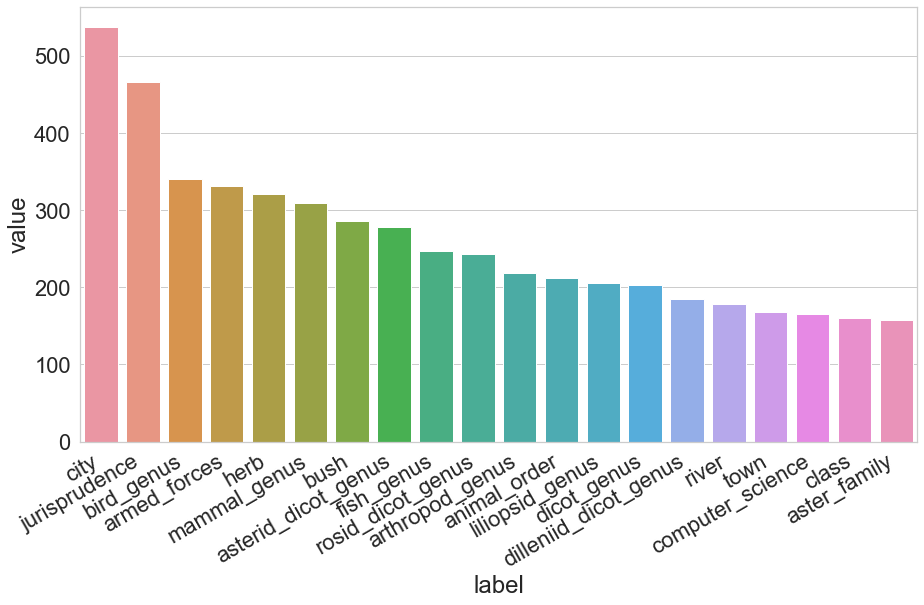
\includegraphics[width=1.0\linewidth, height=0.6\linewidth]{Wordnet_Object_Counts}
		\captionsetup{justification=centering}
		\caption{WordNet}
	\end{subfigure}
	\begin{subfigure}[b]{.5\linewidth}
   		\centering
		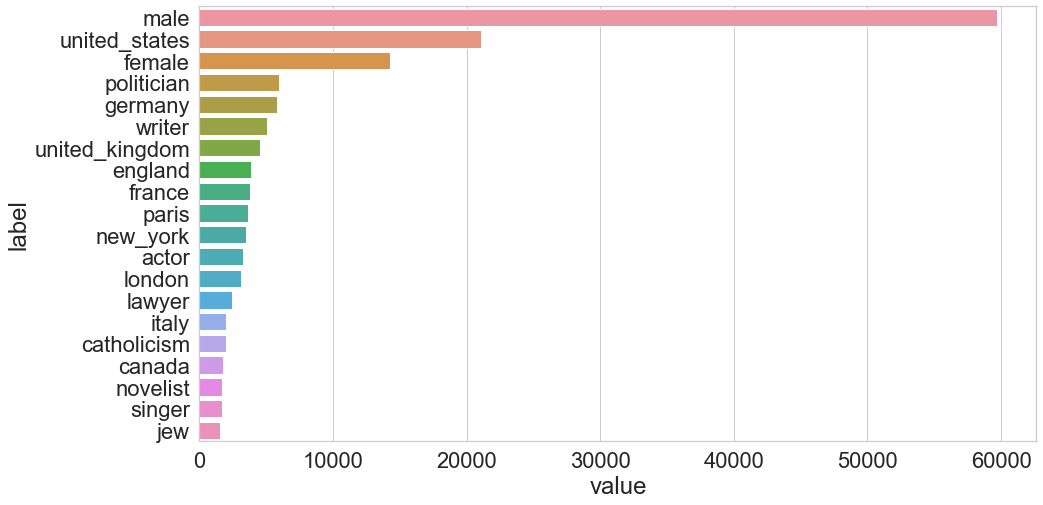
\includegraphics[width=1.0\linewidth, height=0.6\linewidth]{Freebase_Object_Counts}
		\captionsetup{justification=centering}
		\caption{Freebase}
	\end{subfigure}
	\captionsetup{justification=centering}
	\caption{Histogram showing the number of times the 20 most frequent object labels occur in KG facts, in the WordNet and Freebase link prediction datasets.}
\end{figure}

\begin{table}[H]
	\begin{center}
	\begin{tabular}{|l|ccc|ccc|}
		\hline
 		& \multicolumn{3}{c|}{\textbf{WordNet}} & \multicolumn{3}{c|}{\textbf{Freebase}} \\
		& subject & predicate & object & subject & predicate & object \\
		\hline 
		Count & 32,270 & 11 & 33,011 & 67,393 & 13 & 15,342 \\
		Max & 619 & 43,312 & 537 & 37 & 73,897 & 59,663 \\
		Min & 1 & 1,229 & 1 & 1 & 4,464 & 1 \\
		Median & 2 & 7,705 & 3 & 5 & 21,149 & 3 \\
		IQR & 2 & 7,258 & 2 & 4 & 34,033 & 6 \\
		\hline 
	\end{tabular}
	\end{center}
	\captionsetup{justification=centering}
	\caption{Statistics of the WordNet and Freebase link prediction datasets. We show counts of unique subject, predicate and object labels, as well as the maximum, minimum, median and interquartile range of label occurrences.}
\end{table}

\noindent For WordNet, it can be seen that predicates are skewed toward "has instance" with $ 43, 312 $ occurrences, and "type of" with $ 36, 659 $ occurrences. Freebase predicates are somewhat more uniform, however four predicates have occurrences under $ 10, 000 $. \par

\noindent WordNet and Freebase subjects are somewhat uniform, although the median number of occurrences is 2 and 5 respectively, with an interquartile range (IQR) of $ 2 $ and $ 4 $ respectively. WordNet object occurrences are somewhat uniform while Freebase object occurrences are skewed, with a single object, "male" occurring $ 59, 663 $ times, representing $15, 88\% $ of facts. This is in comparison to a median object occurrence of $ 3 $ and an IQR of $ 6 $. \par

\noindent The WordNet dataset is split into a training, validation and test sets of $ 110, 362 \; (80.8 \%) $, $ 5, 215 \; (3.8 \%) $ and $ 21, 034 \; (15.4 \%) $ triples respectively.\ And the Freebase dataset is split into a training, validation and test sets of $ 316, 232 \; (84.2 \%) $, $ 11, 815 \; (3.1 \%) $ and $ 47, 452 \; (12.6 \%) $ triples respectively. 

\subsection{Baseline training algorithm}

\textbf{Model summary.} Our baseline model for this section is inspired by recursive networks (RCNs). The NTN is a bilinear tensor product between the subject, predicate and object, added to an RCN composition of the subject and object. It computes relational scores between pairs of entities. \par

\noindent \textbf{Contrastive max-margin loss.} The contrastive max-margin loss is used to train the NTN model. A relational score is computed for the target triple containing a subject, predicate and object. A relational score is then computed for the same subject and predicate, along with a non-related entity randomly selected and presented as a corrupt object. Relational scores in the range $ (-1, \; 1) $ are produced for the target and corrupt objects, respectively. The training task is to compute a large value for the target score, and small value for the corrupt score. The computed loss is backpropagated through the network to update model parameters. 


%********************************** %Optimised training algorithm **************************************

\subsection{Optimised training algorithm}

\textbf{Implementation.}\ We use the TensorFlow framework \unskip~\citep{abadi2016tensorflow} to implement our NTN training algorithms.\ The NTN model introduced by Chen et al. \unskip ~\citep{socher2013reasoning} and reimplemented in TensorFlow by Doss et al. \unskip ~\citep{Doss2015}, serves as the baseline model. We update the baseline's training algorithm by including early stopping, adaptive moment estimation (Adam) optimisation and hyperparameter random search. We also make use of the same pre-trained word vectors \unskip ~\citep{turian2010word} used to initialise entity and relational embeddings.\ The embedding parameters are adjusted during training to generate latent representations specific to a KG. The models in this section were trained on a MacBook Pro 2015 with 8 cores, 16GB RAM, and 512GB SSD, and no GPU acceleration. We evaluate the models by ranking the accuracy scores of the predicted triples for the respective test sets of WordNet and Freebase. \par

\noindent \textbf{Code to reproduce.} In the interest of reproducibility, all code needed to train and test the models in this section can be found at the following links. \newline
Baseline NTN: \url{https://github.com/xhosaBoy/recursive-neural-tensor-networks} \newline
Optimised NTN: \url{https://github.com/xhosaBoy/optimised-neural-tensor-network} 

\subsubsection{Results} 
The accuracy results of the NTN model trained using the original baseline training algorithm, compared to the optimised training algorithm are presented in Figure 4.8, as well as Table 4.2. The hypothesis outperforms the baseline accuracy across both KGs, and It significantly outperforms the baseline on the WordNet KG. Hyperparameter random search seems to be responsible for this improvement, as the hypothesis begins outperforming the baseline from the first epoch. \ All experiments were only able to complete a maximum of $ 12 $ epochs before overwhelming compute resources. 

\bigskip
\bigskip

\begin{figure}[H]
	\begin{subfigure}[b]{.5\linewidth}
   		\centering
    		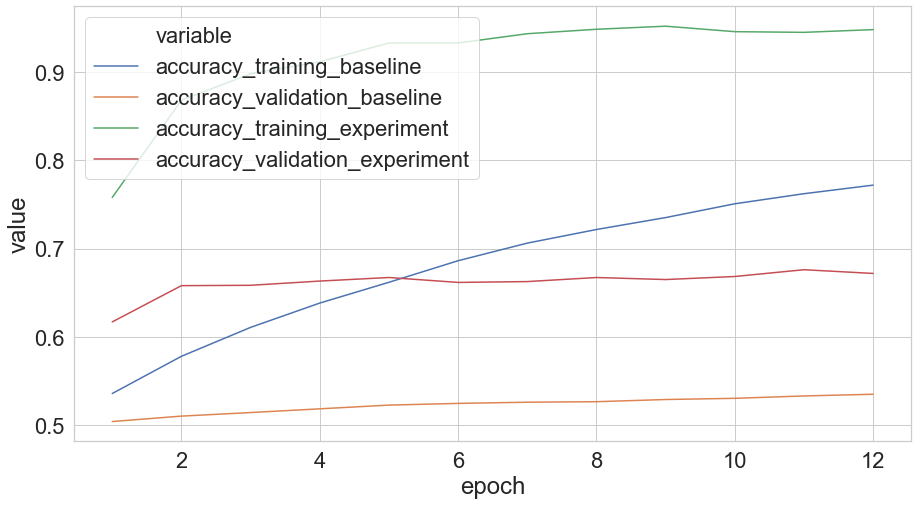
\includegraphics[width=1.0\linewidth, height=0.6\linewidth]{Wordnet_Accuracy_Results_Early_Stopping}
		\captionsetup{justification=centering}
		\caption{WordNet}
	\end{subfigure}
	\begin{subfigure}[b]{.5\linewidth}
   		\centering
		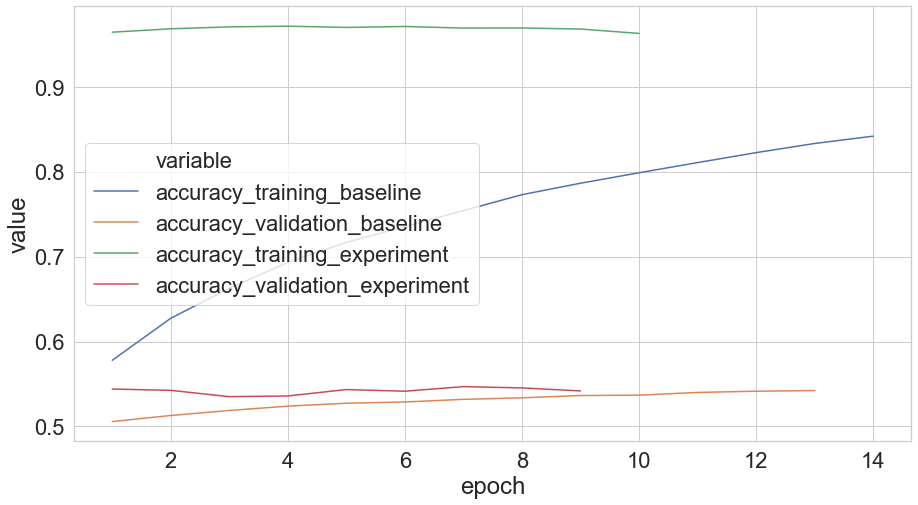
\includegraphics[width=1.0\linewidth, height=0.6\linewidth]{Freebase_Accuracy_Results}
		\captionsetup{justification=centering}
		\caption{Freebase}
	\end{subfigure}
	\captionsetup{justification=centering}
	\caption{Training and validation accuracy vs training epochs for the two datasets. The optimised algorithm performs significantly better, especially on WordNet.}
\end{figure}

\begin{table}[H]
	\centering
	\begin{tabular}{lllllllllll}
  		\textbf{Model} & \textbf{WordNet} & \textbf{Freebase} & \textbf{Avg} \\
  		\hline
  		Original NTN \unskip ~\citep{socher2013reasoning} & \textbf{.862} & \textbf{.900} & \textbf{.881} \\
  		Reimplemented NTN baseline  \unskip ~\citep{Doss2015} & .562 & .535 & .549 \\
  		\hline
  		Optimised NTN (ours) & .674 & .548 & .611 \\
		&
	\end{tabular}
	\captionsetup{justification=centering}
	\caption{Link prediction accuracy on WordNet and Freebase KG test sets. Our reimplemented NTN with the optimised training algorithm outperforms the baseline NTN, but the original NTN algorithm significantly outperforms all models. This may be due to differences in other training algorithm properties such as number of epochs and hyperparameter values.}
\end{table}


%********************************** %HypER and Covariate Shift  **************************************

\section{HypER and HypER+}

\subsection{Datasets} 
For the second set of experiments we use the WN18 \citep{bordes2013translating} and FB15k \citep{bordes2013translating} link prediction benchmark datasets.\ WN18 is a subset of WordNet, containing $ 40, 943 $ entities, $ 18 $ relations and 151,442 triples. FB15k is a subset of Freebase, containing $ 14, 951 $ entities, $ 1, 345 $ relations and 592,213 triples. Visualisations of the respective KGs, as well as a sample of RDF triple encoded facts, are presented in Figures 4.9 to 4.12.\ KG summary statistics are presented in Figures 4.13 to 4.16, and Table 4.3. 

\begin{figure}
   	\centering
    	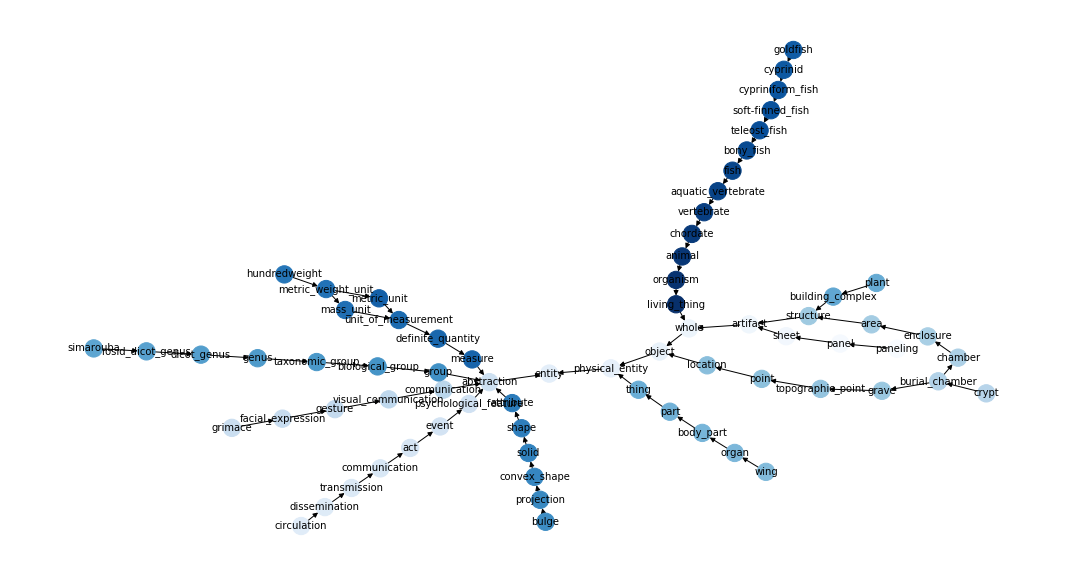
\includegraphics[width=0.9\textwidth, height=0.6\textwidth]{WN18_Graph}
	\captionsetup{justification=centering}
	\caption{A subset of WN18 facts structured as a KG. Entities are nodes, and relations are edges, where facts are encoded as RDF triples.}
\end{figure}

\begin{figure}
   	\centering
    	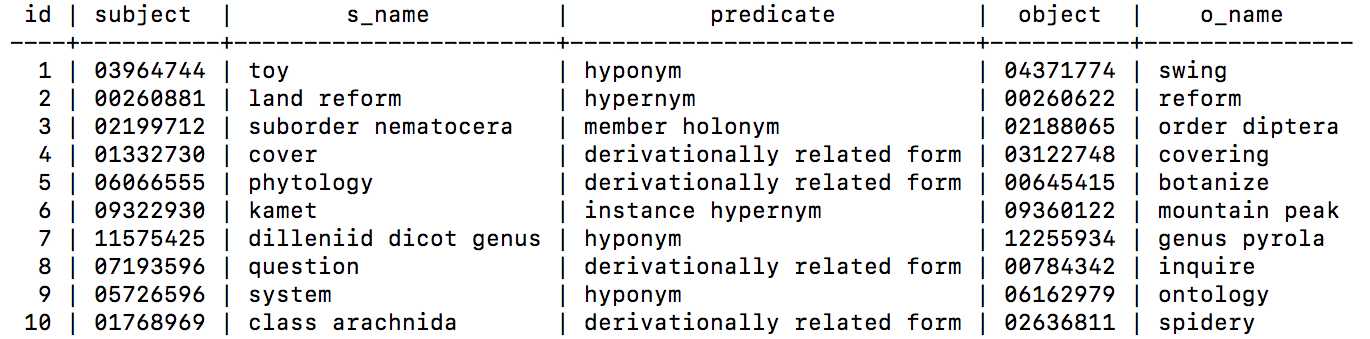
\includegraphics[width=0.9\textwidth, height=0.3\textwidth]{wn18_fact_sample}
	\captionsetup{justification=centering}
	\caption{A sample of RDF triples from the WN18 KG.}
\end{figure}

\begin{figure}
   	\centering
    	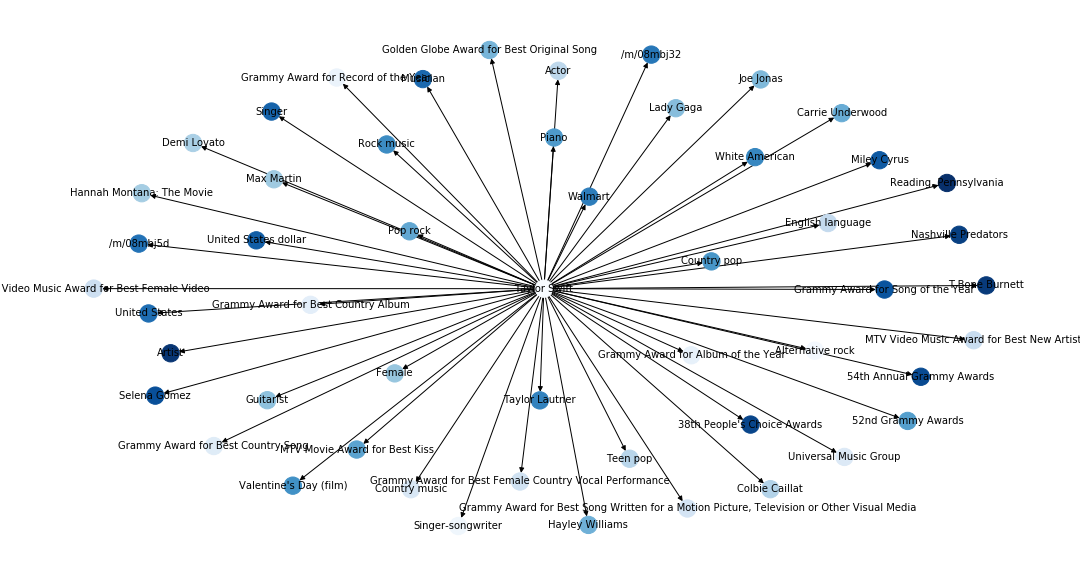
\includegraphics[width=0.9\textwidth, height=0.6\textwidth]{FB15k_Graph}
	\captionsetup{justification=centering}
	\caption{A subset of FB15k facts structured as a KG. Entities are nodes, and relations are edges, where facts are encoded as RDF triples.}
\end{figure}

\begin{figure}
   	\centering
    	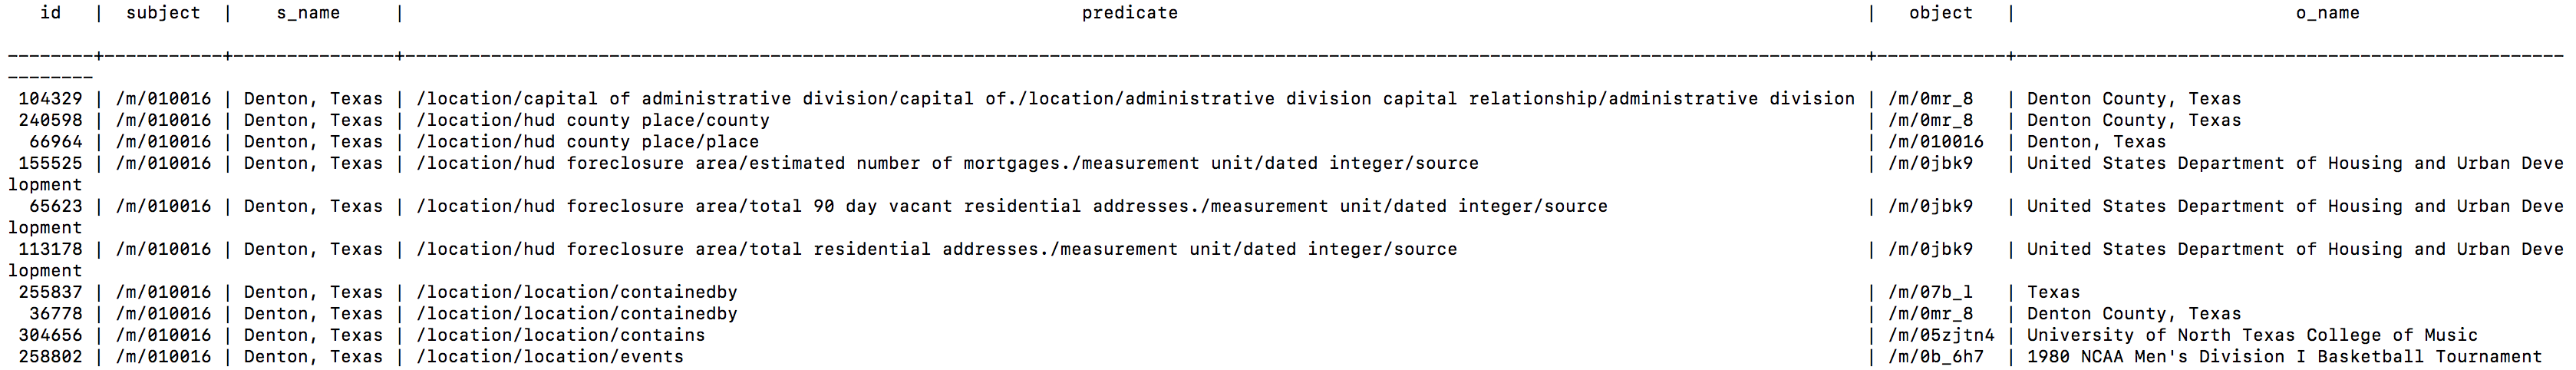
\includegraphics[width=1.0\textwidth, height=0.4\textwidth]{fb15k_fact_sample}
	\captionsetup{justification=centering}
	\caption{A sample of RDF triples from the FB15k KG.}
\end{figure}


%********************************** %Subject **************************************

\begin{figure}
	\begin{subfigure}[b]{.5\linewidth}
   		\centering
    		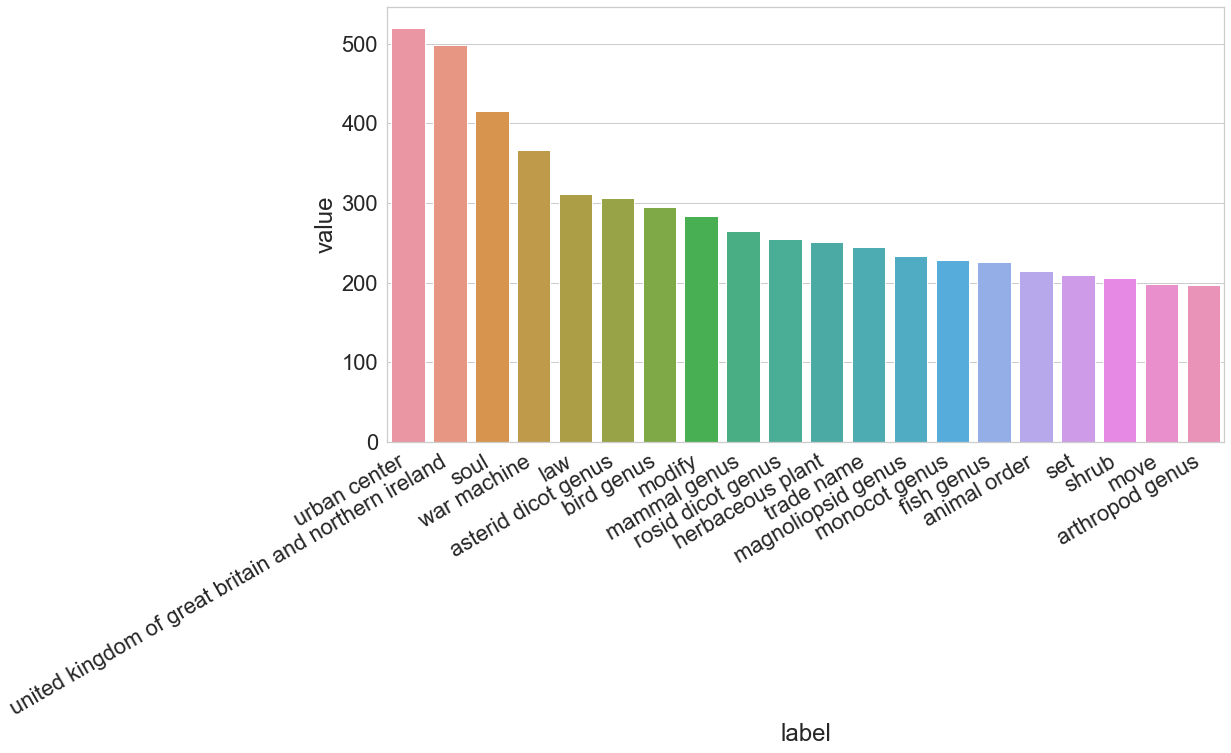
\includegraphics[width=1.0\linewidth, height=0.7\linewidth]{WN18_Subject_Counts}
		\captionsetup{justification=centering}
		\caption{WN18}
	\end{subfigure}
	\begin{subfigure}[b]{.5\linewidth}
   		\centering
		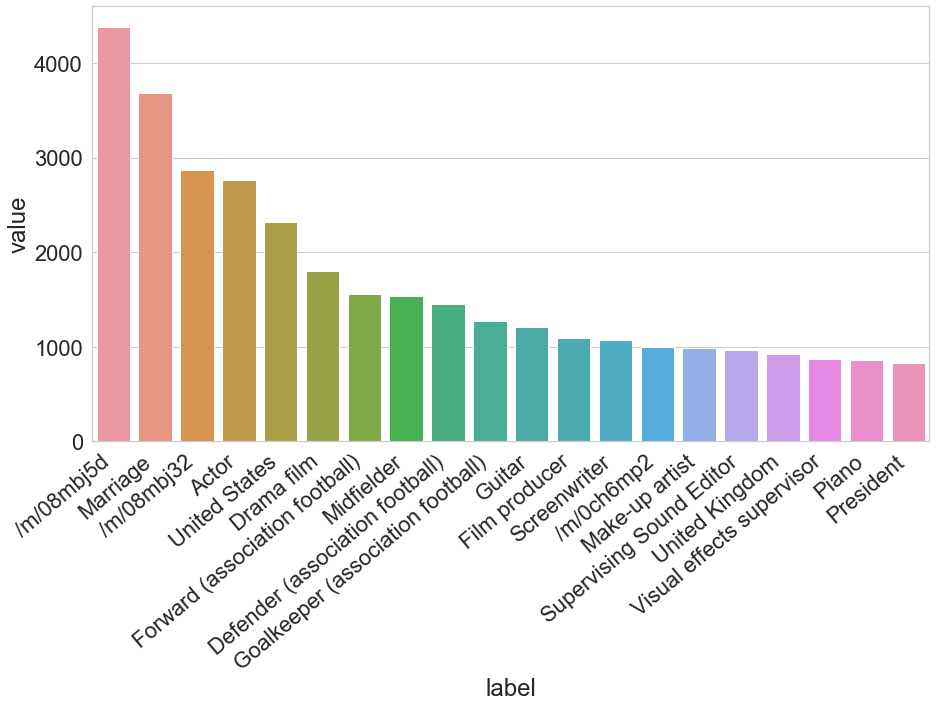
\includegraphics[width=1.0\linewidth, height=0.7\linewidth]{FB15k_Subject_Counts}
		\captionsetup{justification=centering}
		\caption{FB15k}
	\end{subfigure}
	\captionsetup{justification=centering}
	\caption{Histogram showing the number of times the 20 most frequent subject labels occur in KG facts, in the WN18 and FB15k link prediction datasets.}
\end{figure}


%********************************** %Predicate  **************************************

\begin{figure}
   	\centering
    	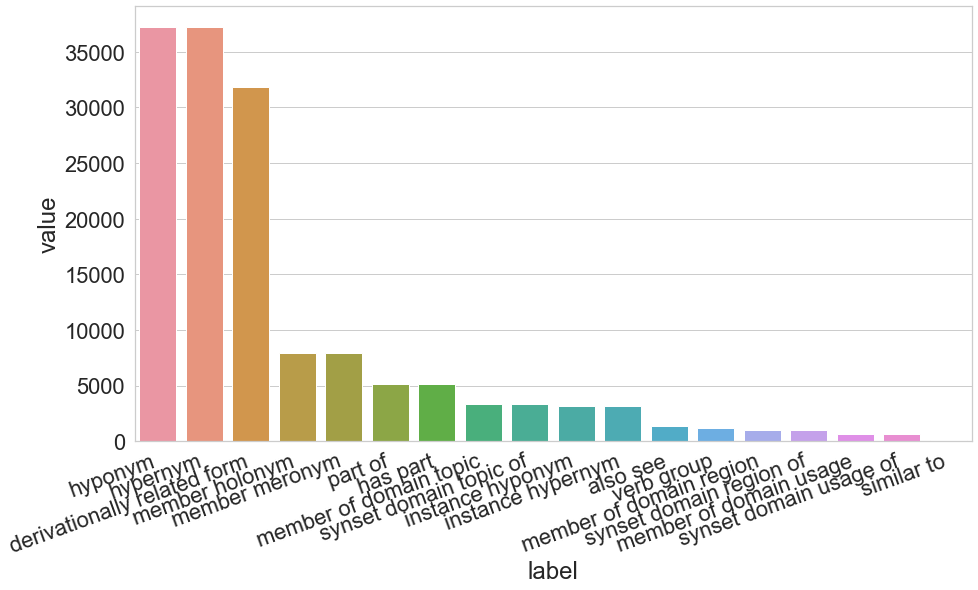
\includegraphics[width=0.7\textwidth, height=0.3\textheight]{WN18_Predicate_Counts}
	\captionsetup{justification=centering}
	\caption{Histogram showing the number of times predicate labels occur in KG facts, in the WN18 link prediction dataset.}
\end{figure}

\begin{figure}
   	\centering
    	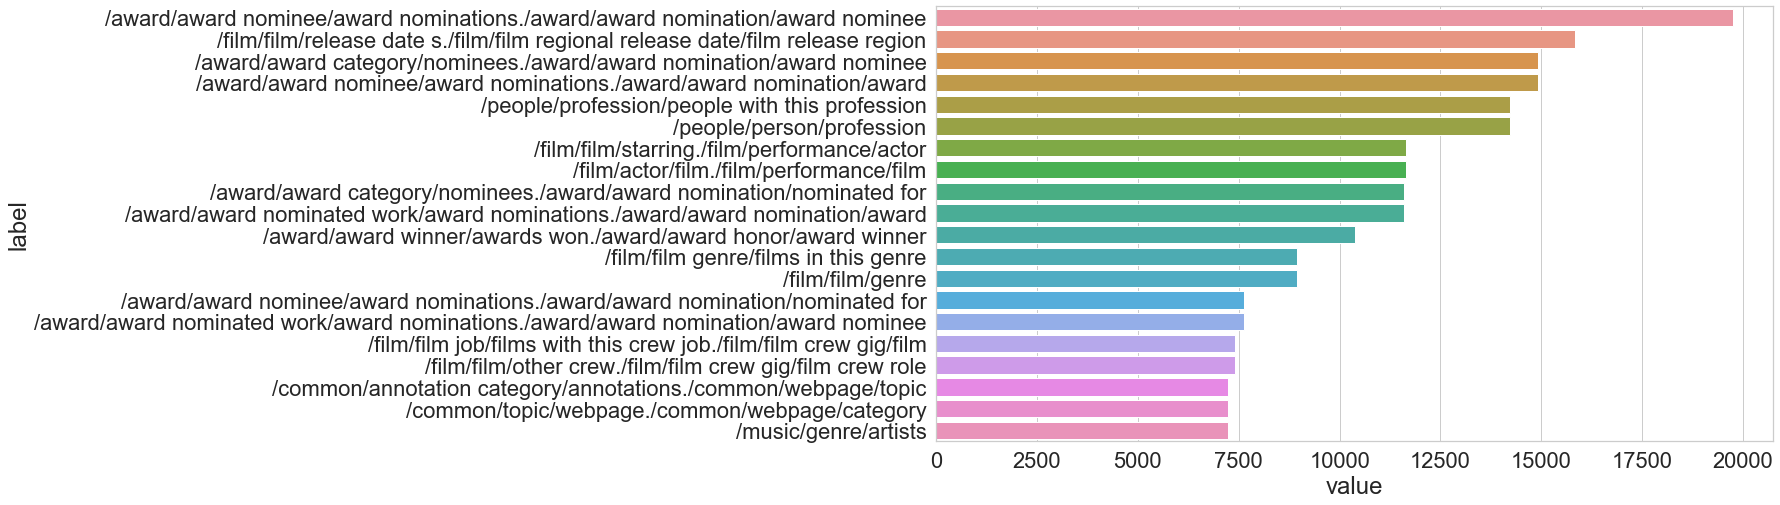
\includegraphics[width=1.0\textwidth, height=0.3\textheight]{FB15k_Predicate_Counts}
	\captionsetup{justification=centering}
	\caption{Histogram showing the number of times the 20 most frequent predicate labels occur in KG facts, in the FB15k link prediction dataset.}
\end{figure}


%********************************** %Object  **************************************

\begin{figure}
	\begin{subfigure}[b]{.5\linewidth}
   		\centering
    		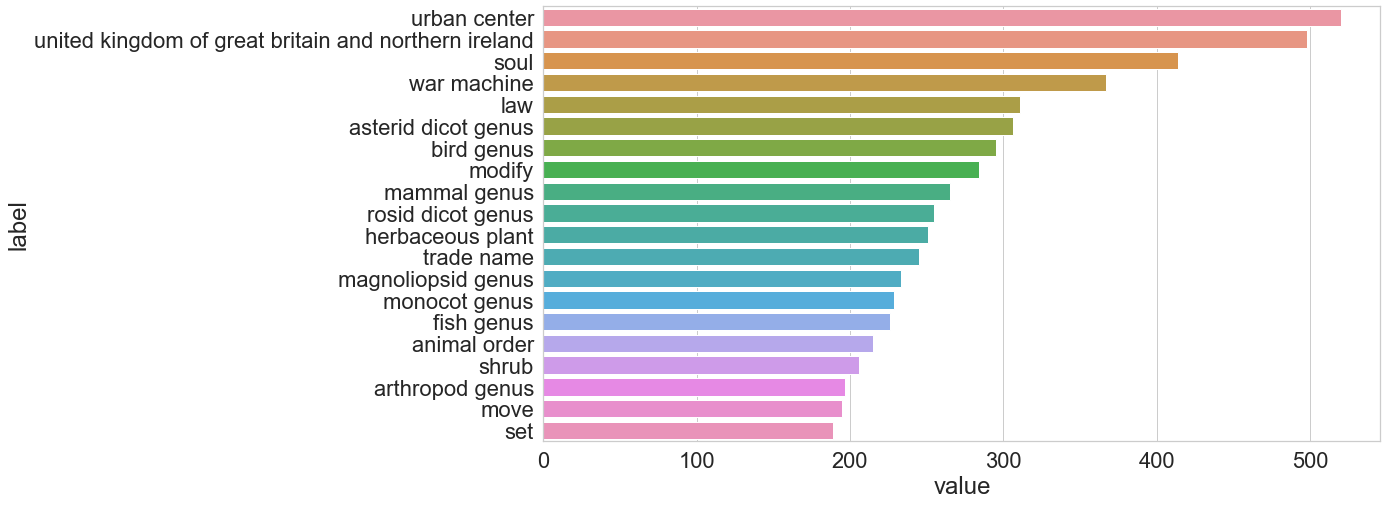
\includegraphics[width=1.0\linewidth, height=0.7\linewidth]{WN18_Object_Counts}
		\captionsetup{justification=centering}
		\caption{WN18}
	\end{subfigure}
	\begin{subfigure}[b]{.5\linewidth}
   		\centering
		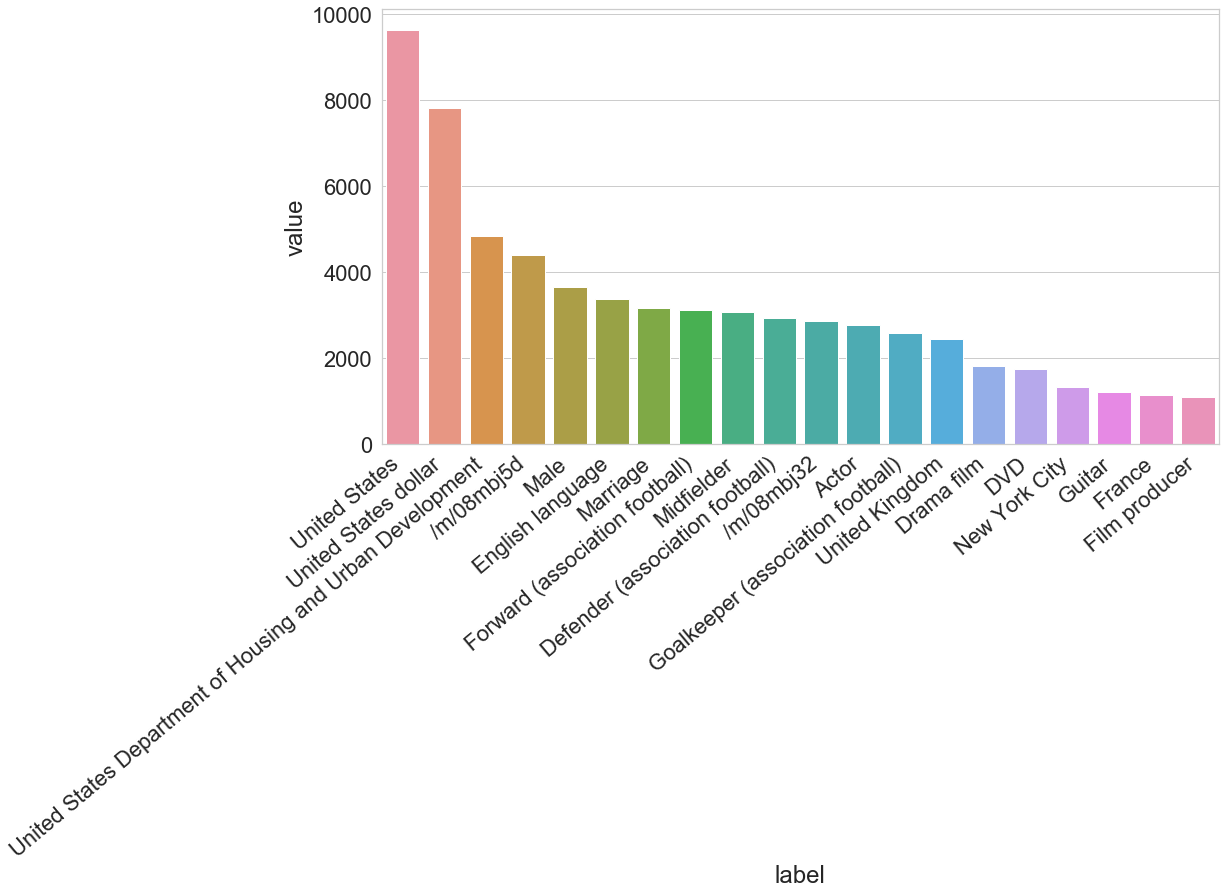
\includegraphics[width=1.0\linewidth, height=0.7\linewidth]{FB15k_Object_Counts}
		\captionsetup{justification=centering}
		\caption{FB15k}
	\end{subfigure}
	\captionsetup{justification=centering}
	\caption{Histogram showing the number of times the 20 most frequent object labels occur in KG facts, in the WN18 and FB15k link prediction datasets.}
\end{figure}

\begin{table}[H]
	\begin{center}
	\begin{tabular}{|l|ccc|ccc|}
		\hline
 		& \multicolumn{3}{c|}{\textbf{WN18}} & \multicolumn{3}{c|}{\textbf{FB15k}} \\
		& subject & predicate & object & subject & predicate & object \\
		\hline 
		Count & 32,544 & 18 & 32,543 & 14,865 & 1,345 & 14,930 \\
		Max & 520 & 37,221 & 520 & 4,381 & 19,764 & 9,645 \\
		Min & 1 & 86 & 1 & 1 & 1 & 1 \\
		Median & 3 & 3,243 & 3 & 27 & 26 & 23 \\
		IQR & 2 & 6,191 & 2 & 32 & 166 & 30 \\
		\hline 
	\end{tabular}
	\end{center}
	\captionsetup{justification=centering}
	\caption{Statistics of the WN18 and FB15k link prediction datasets. We show counts of unique subject, predicate and object labels, as well as the maximum, minimum, median and interquartile range of label occurrences.}
\end{table}

\noindent For WN18, it can be seen that predicates are skewed toward the relations "hyponym",  "hypernym", and "derivationally related from", with a maximum of $ 37, 221 $ occurrences. FB15k predicates are somewhat more uniform. \par

\noindent WN18 and FB15k subjects are somewhat uniform aside from a small number of high occurring entities, with the median number of occurrences being $ 3 $ and $ 27 $ respectively, and with an IQR of $ 2 $ and $ 32 $ respectively.\ WN18 object occurrences are somewhat uniform.\ FB15k object occurrences are skewed, with the "United States" partaking in the highest number of triples.\ This is in comparison to a median object occurrence of $ 23 $ and an IQR of 30. \par

\noindent The WN18 dataset is split into a training, validation and test sets of $ 141, 442 \; (93.4 \%) $, $ 5, 000 \; (3.3 \%) $ and $ 5, 000 \; (3.3 \%) $ triples respectively.\ The FB15k dataset is split into a training, validation and test sets of $ 483, 142 \; (81.6 \%) $, $ 50, 000 \; (8.4 \%) $ and $ 59, 071 \; (10.0 \%) $ triples, respectively. 

\subsection{Baseline algorithm}
\textbf{Model summary.} HypER is a model that takes the convolution between a predicate-specific filter and subject vector, to generate a subject-predicate feature map. This map is flattened and passed through a nonlinearity, before an inner product is taken with an object vector. The result is a relational score which is passed through a logistic sigmoid to generate a probability of a potential relationship between pairs of entities. \par

\noindent \textbf{Binary cross-entropy loss.} The binary cross-entropy loss is used to train HypER. Like the NTN model, the input consists of a subject-predicate pair, and an object is presented as a target to complete the triple. A relational score is generated for each sample and passed through a logistic sigmoid. Loss is generated by comparing the produced likelihood with the expected likelihood, $ 0 $ or $ 1 $. The sum of losses in a batch of samples is aggregated and backpropagated through the network for parameter update. \par

\noindent \textbf{Benchmark metrics.} The current suite of link prediction benchmark metrics includes Hit@10, Hit@3, Hit@1, Mean Rank, and Mean Reciprocal Rank.\ For these models, all objects in the KG are assigned a probability and then ranked in descending order. The Hit@X metrics comprise the relation prediction accuracy measures of the model, where X describes the lowest rank the predicted object can occupy. For example in Hit@10, only the top 10 objects are considered as accurate. The Mean Rank is the average predicted object rank Hit@1 and can be measured after any training epoch. The Mean Reciprocal Rank is the inverse of the Mean Rank. \par


%********************************** %HypER+  **************************************

\subsection{HypER+}

\textbf{Implementation.} Here we use the PyTorch framework to develop our model. The HypER model introduced by Bala\u{z}ev\'{i}c et al. \unskip ~\citep{balazevic2019hypernetwork} serves as a baseline. We apply batch normalisation to the hypernetwork input layer and thus introduce HypER+. Entity and relational embeddings are randomly initialised during model training. These embeddings are dynamically adjusted during the training process to generate latent representations specific to a KG. The models in this section were trained on Google Cloud Platform, on an N1 series instance with  8 CPU cores, 30GB RAM, 512GB SSD and an Nvidia Tesla P100 GPU. We train the respective models for $ 500 $ epoch, and evaluate them using the test sets of WN18 and FB15k. \par

\noindent \textbf{Code to reproduce.} In the interest of reproducibility, all code needed to train and test the models in this section can be found at the following links. \newline
Baseline HypER: \url{https://github.com/xhosaBoy/HypER-baseline} \newline
HypER+: \url{https://github.com/xhosaBoy/HypER-normalised-relations} 

\subsubsection{Results}
Results based on current standard link prediction metrics (Hit@10, Hit@3, Hit@1, Mean Rank and Mean Reciprocal Rank) for the Hyper+ model compared against the HypER model baseline, are presented in Figures 4.17 to 4.19, as well as Tables 4.4 and 4.5. T-SNE analysis \unskip ~\citep{maaten2008visualizing} of HypER+ on the FB15k KG is presented in Figures 4.20 to 4.23. \par

\noindent HypER+ achieves near-identical results with the HypER baseline on the WN18 KG across all metrics, and significantly outperforms the HypER baseline on the FB15k KG. The impact of hypernetwork batch normalisation is pronounced, perhaps due to the upstream influence of predicate input covariate shift. 

\bigskip
\bigskip


%********************************** %Hits@10  **************************************

\begin{figure}[H]
	\begin{subfigure}[b]{.5\linewidth}
   		\centering
    		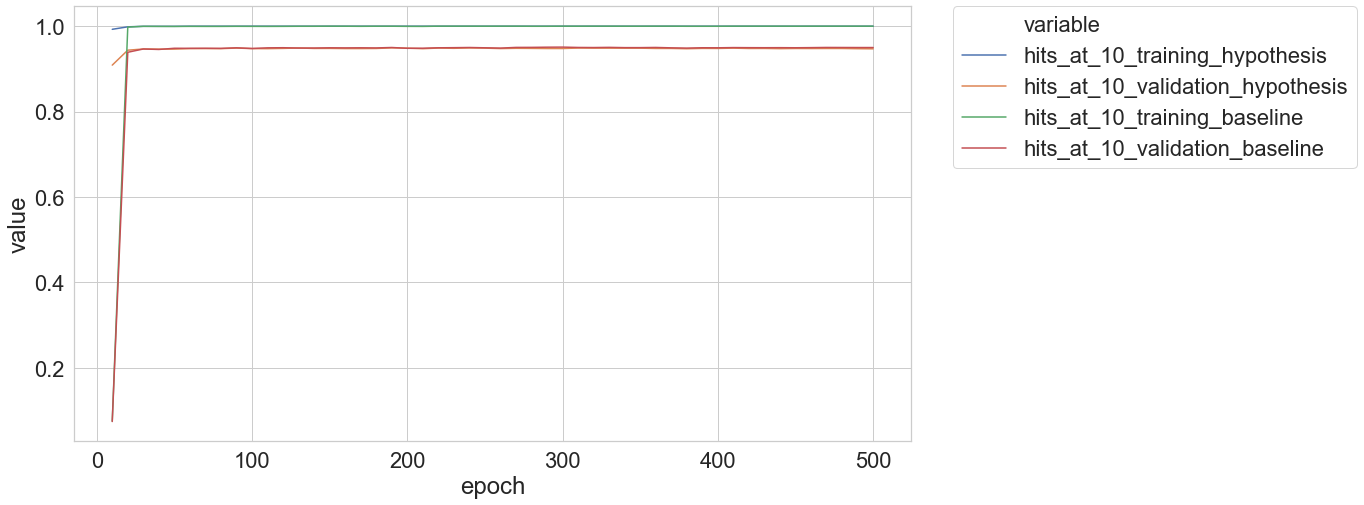
\includegraphics[width=1.0\linewidth, height=0.6\linewidth]{WN18_hits_at_10_Results}
		\captionsetup{justification=centering}
		\caption{WN18}
	\end{subfigure}
	\begin{subfigure}[b]{.5\linewidth}
   		\centering
		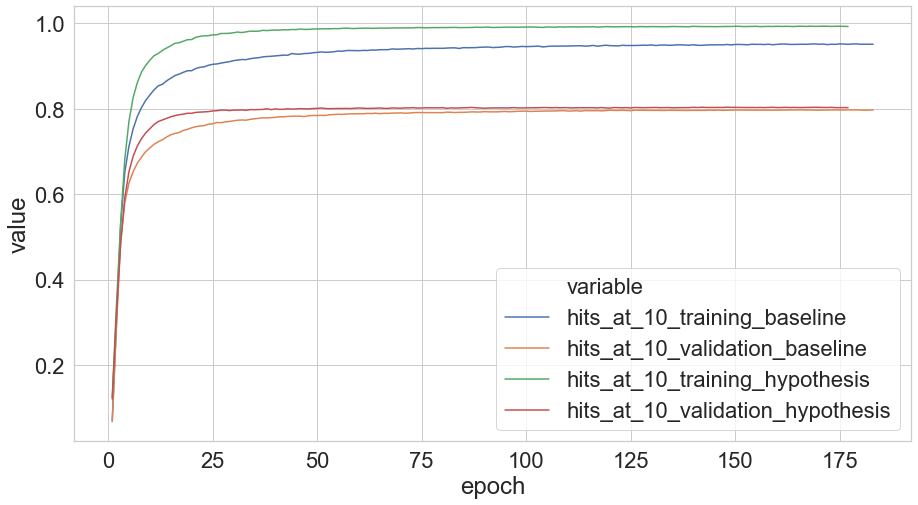
\includegraphics[width=1.0\linewidth, height=0.6\linewidth]{FB15k_hits_at_10_Results}
		\captionsetup{justification=centering}
		\caption{FB15k}
	\end{subfigure}
	\captionsetup{justification=centering}
	\caption{Hit@10 vs training epoch. There is hardly any difference between the hypothesis and baseline models for the WN18 KG. The hypothesis model outperforms the baseline on the FB15k KG, although the validation difference is not as pronounced as the training difference.}
\end{figure}

\bigskip
\bigskip
\bigskip
\bigskip


%********************************** %Hits@3  **************************************

\begin{figure}[H]
	\begin{subfigure}[b]{.5\linewidth}
   		\centering
    		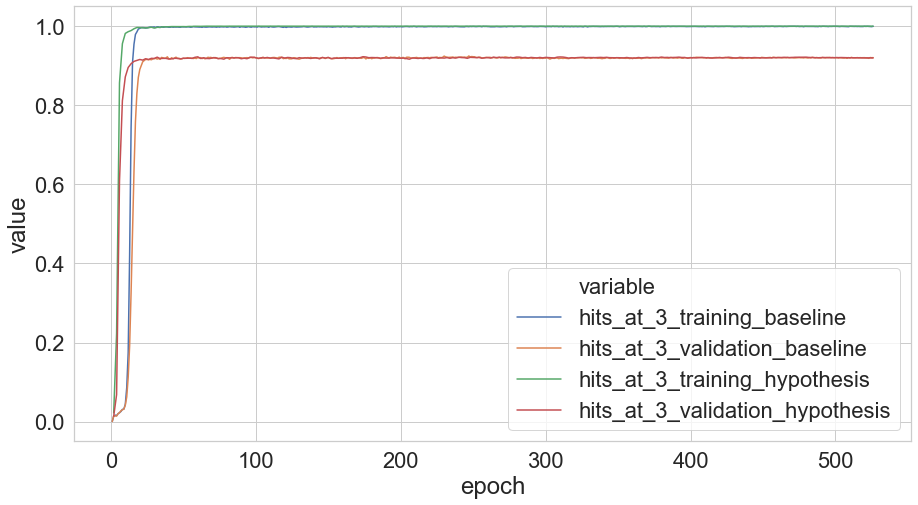
\includegraphics[width=1.0\linewidth, height=0.6\linewidth]{WN18_hits_at_3_Results}
		\captionsetup{justification=centering}
		\caption{WN18}
	\end{subfigure}
	\begin{subfigure}[b]{.5\linewidth}
   		\centering
		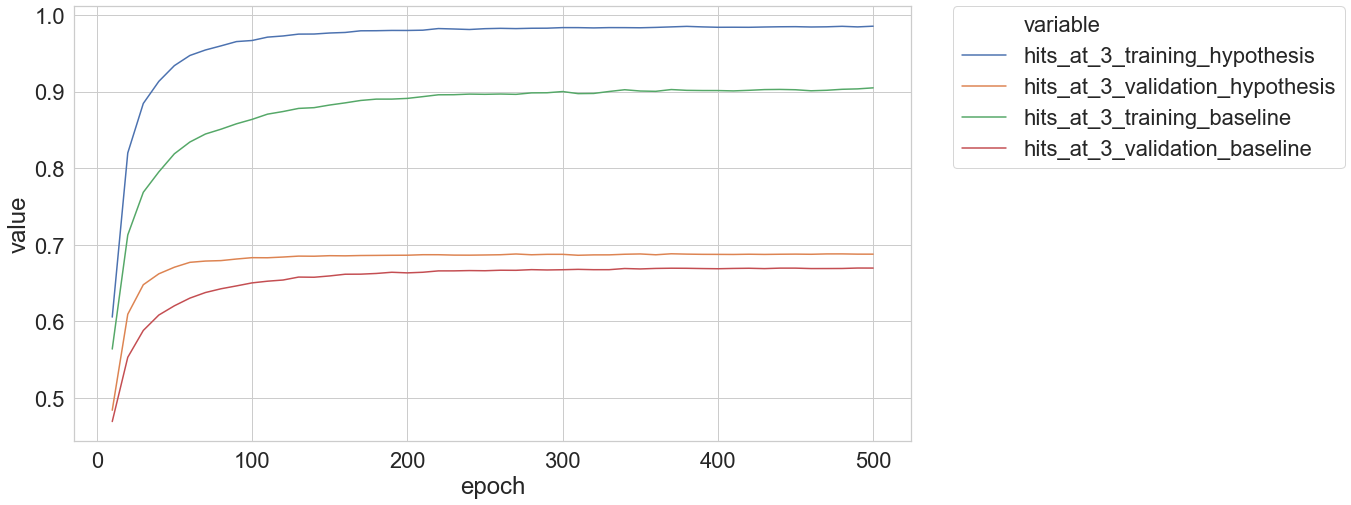
\includegraphics[width=1.0\linewidth, height=0.6\linewidth]{FB15k_hits_at_3_Results}
		\captionsetup{justification=centering}
		\caption{FB15k}
	\end{subfigure}
	\captionsetup{justification=centering}
	\caption{Hit@3 vs training epoch. The models have similar behaviour to the Hit@10 metric, and both have lower accuracy. There is however a larger performance difference between the hypothesis and baseline. This may be due to the more robust generalisation requirements with a smaller subset of acceptable answers, resulting in a more pronounced impact from covariate shift of latent predicate parameters.}
\end{figure}


%********************************** %Hits@1  **************************************

\begin{figure}[H]
	\begin{subfigure}[b]{.5\linewidth}
   		\centering
    		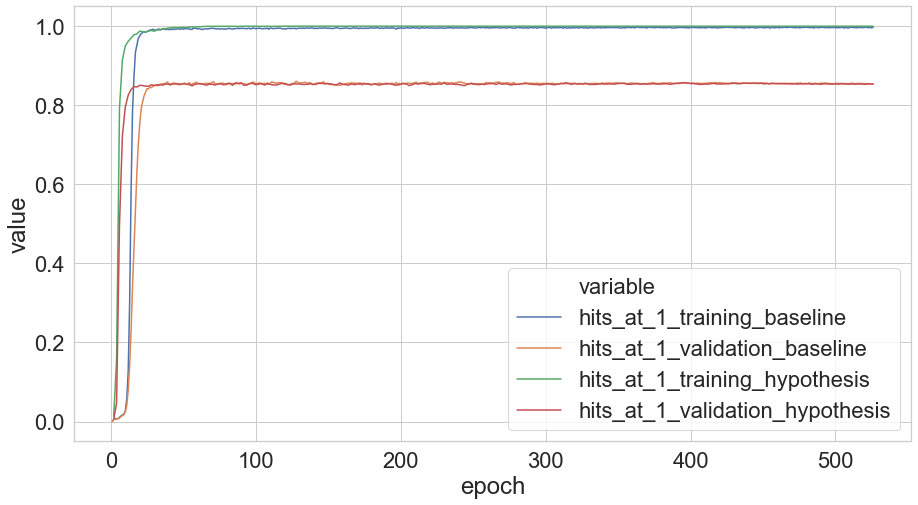
\includegraphics[width=1.0\linewidth, height=0.6\linewidth]{WN18_hits_at_1_Results}
		\captionsetup{justification=centering}
		\caption{WN18}
	\end{subfigure}
	\begin{subfigure}[b]{.5\linewidth}
   		\centering
		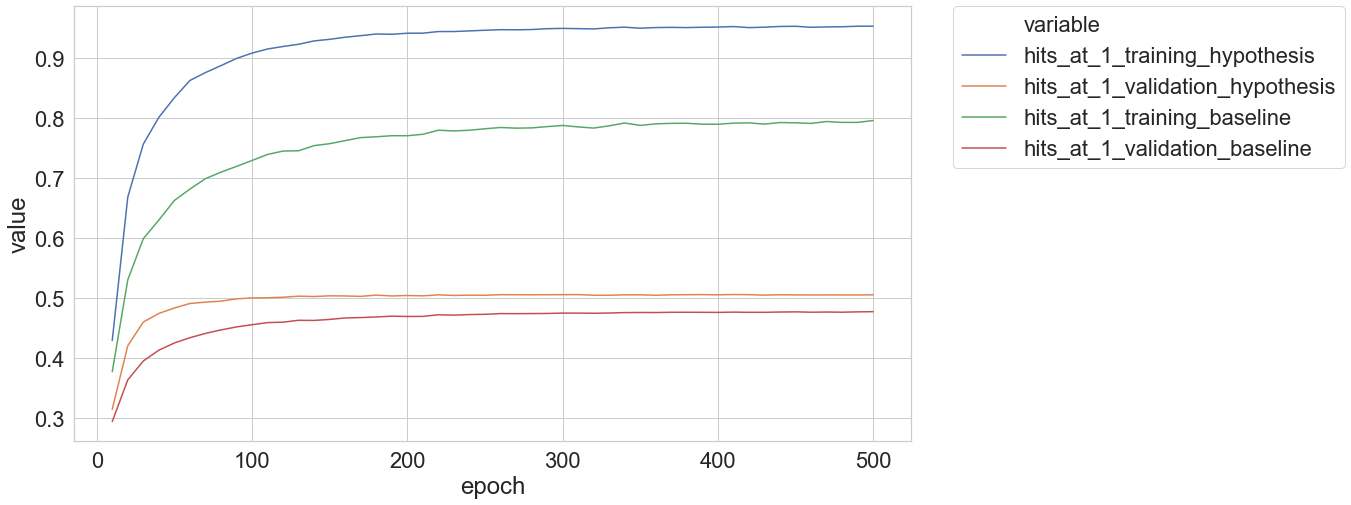
\includegraphics[width=1.0\linewidth, height=0.6\linewidth]{FB15k_hits_at_1_Results}
		\captionsetup{justification=centering}
		\caption{FB15k}
	\end{subfigure}
	\captionsetup{justification=centering}
	\caption{Hit@1 vs training epoch. The models have similar behaviour to the Hit@10 and Hit@3 metrics, and both have even lower accuracy. There is no discernible difference between the models on the WN18 KG, however there is once again a larger difference between them on the FB15k KG. }
\end{figure}

\bigskip
\bigskip
\bigskip
\bigskip


%********************************** %Test results **************************************

\begin{table}[H]
		\centering
		\begin{tabular}{lllllllllll}
  			\textbf{Model} & \textbf{H@10} & \textbf{H@3} & \textbf{H@1} & \textbf{MR} & \textbf{MRR} \\
  			\hline
  			TransE \unskip~\citep{bordes2013translating} & .892 & - & - & \textbf{251} & - \\
  			DistMult \unskip~\citep{yang2014embedding} & .936 & .914 & .728 & 902 & .822 \\
  			ComplEx \unskip~\citep{trouillon2016complex} & .947 & .936 & .936 & - & .941 \\
  			Neural LP \unskip~\citep{yang2017differentiable} & .945 & - & - & - & .940 \\
			R-GCN \unskip~\citep{schlichtkrull2018modeling} & \textbf{.964} & .929 & .697 & - & .819 \\
			TorusE \unskip~\citep{ebisu2018toruse} & .954 & .950 & .943 & - & .947 \\
			ConvE \unskip~\citep{dettmers2018convolutional} & .956 & .946 & .935 & 374 & .943 \\
			HypER \unskip~\citep{balazevic2019hypernetwork} & .958 & \textbf{.955} & \textbf{.947} & 431 & \textbf{.951} \\
  			\hline
  			HypER+ (ours) & .957 & .954 & .946 & 565 & .950 \\
			&
		\end{tabular}
		\captionsetup{justification=centering}
		\caption{Relation prediction test results on WN18. The hypothesis is outperformed by the baseline HypER model across all metrics. It should however be noted that the difference is in the order of $ 0.1\% $, indicating almost identical performance. This is consistent with training and validation results shown earlier. Interestingly, the R-GCN model achieves the highest Hit@10 performance. This model uses the graph modelling SRL paradigm, as opposed to latent feature modelling, and does perform poorly across all other metrics. There may be opportunity in exploring this paradigm further. }
\end{table}

\begin{table}
		\centering
		\begin{tabular}{lllllllllll}
  			\textbf{Model} & \textbf{H@10} & \textbf{H@3} & \textbf{H@1} & \textbf{MR} & \textbf{MRR} \\
  			\hline
  			TransE \unskip~\citep{bordes2013translating} & .471 & - & - & 125 & - \\
  			DistMult \unskip~\citep{yang2014embedding} & .824 & .733 & .546 & 97 & .654 \\
  			ComplEx \unskip~\citep{trouillon2016complex} & .840 & .759 & .599 & - & .692 \\
  			Neural LP \unskip~\citep{yang2017differentiable} & .837 & - & - & - & .760 \\
			R-GCN \unskip~\citep{schlichtkrull2018modeling} & .842 & .760 & .601 & - & .696 \\
			TorusE \unskip~\citep{ebisu2018toruse} & .832 & .771 & .674 & - & .733\\
			ConvE \unskip~\citep{dettmers2018convolutional} & .831 & .723 & .558 & 51 & .657 \\
			HypER \unskip~\citep{balazevic2019hypernetwork} & .885 & .829 & .734 & \textbf{44} & .790 \\
  			\hline
  			HypER+ (ours) & \textbf{.894} & \textbf{.856} & \textbf{.790} & 79 & \textbf{.829} \\
			&
		\end{tabular}
		\captionsetup{justification=centering}
		\caption{Relation prediction test results on FB15k. The hypothesis outperforms the baseline HypER model across all metrics, aside from Mean Rank. Unlike the performance difference on the WN18 KG, the difference here is by a number of percentage points, indicating a significant improvement over the baseline. The hypernetwork approach also significantly outperforms the R-GCN model.}
\end{table}


%********************************** %T-SNE **************************************

\begin{figure}
   	\centering
    	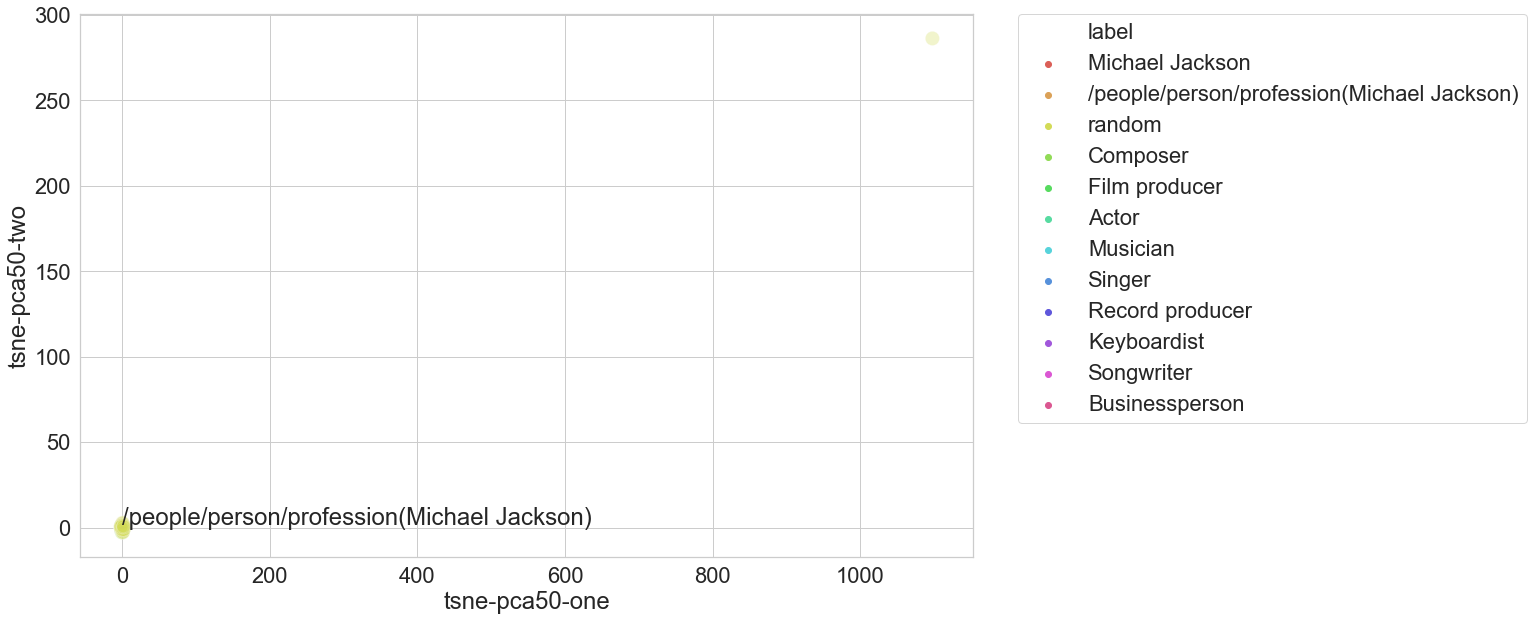
\includegraphics[width=0.7\textwidth, height=0.3\textheight]{t_sne_train_profession}
	\captionsetup{justification=centering}
	\caption{FB15k T-SNE: Triples about "Michael Jackson's" (subject) "profession" (predicate), pre HypER+ training. The legend lists all professions (objects) known to have been performed by Michael Jackson. Most objects in the KG, regardless of type, begin clustered in the same embedding region on the bottom left. This includes the hidden subject-predicate vector,  "/people/person/profession(Michael Jackson)", used to take an inner product with an object.}
\end{figure}

\begin{figure}
   	\centering
    	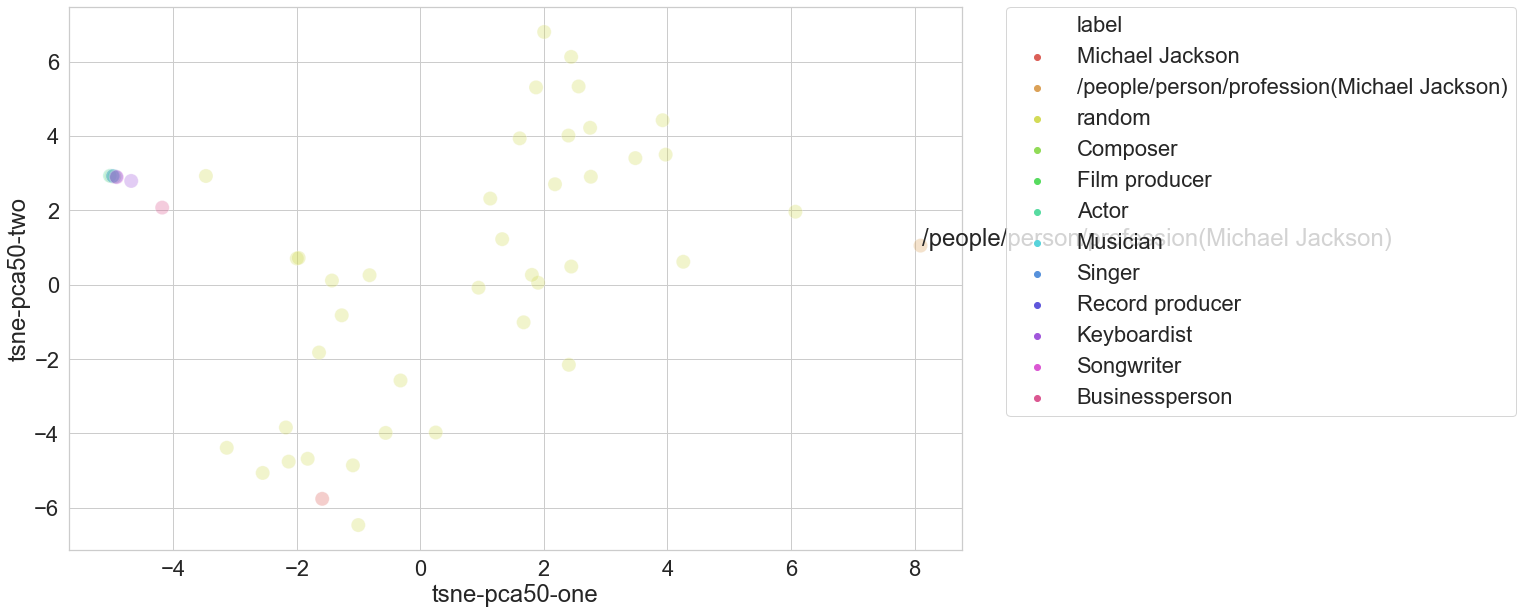
\includegraphics[width=0.7\textwidth, height=0.3\textheight]{t_sne_test_profession}
	\captionsetup{justification=centering}
	\caption{FB15k T-SNE: Triples about "Michael Jackson"'s (subject) profession (predicate), post HypER+ training. Professions Michael Jackson is known to have performed are now all clustered within the same embedding region. This indicates the model has built some conceptual understanding around the objects.}
\end{figure}

\begin{figure}
   	\centering
    	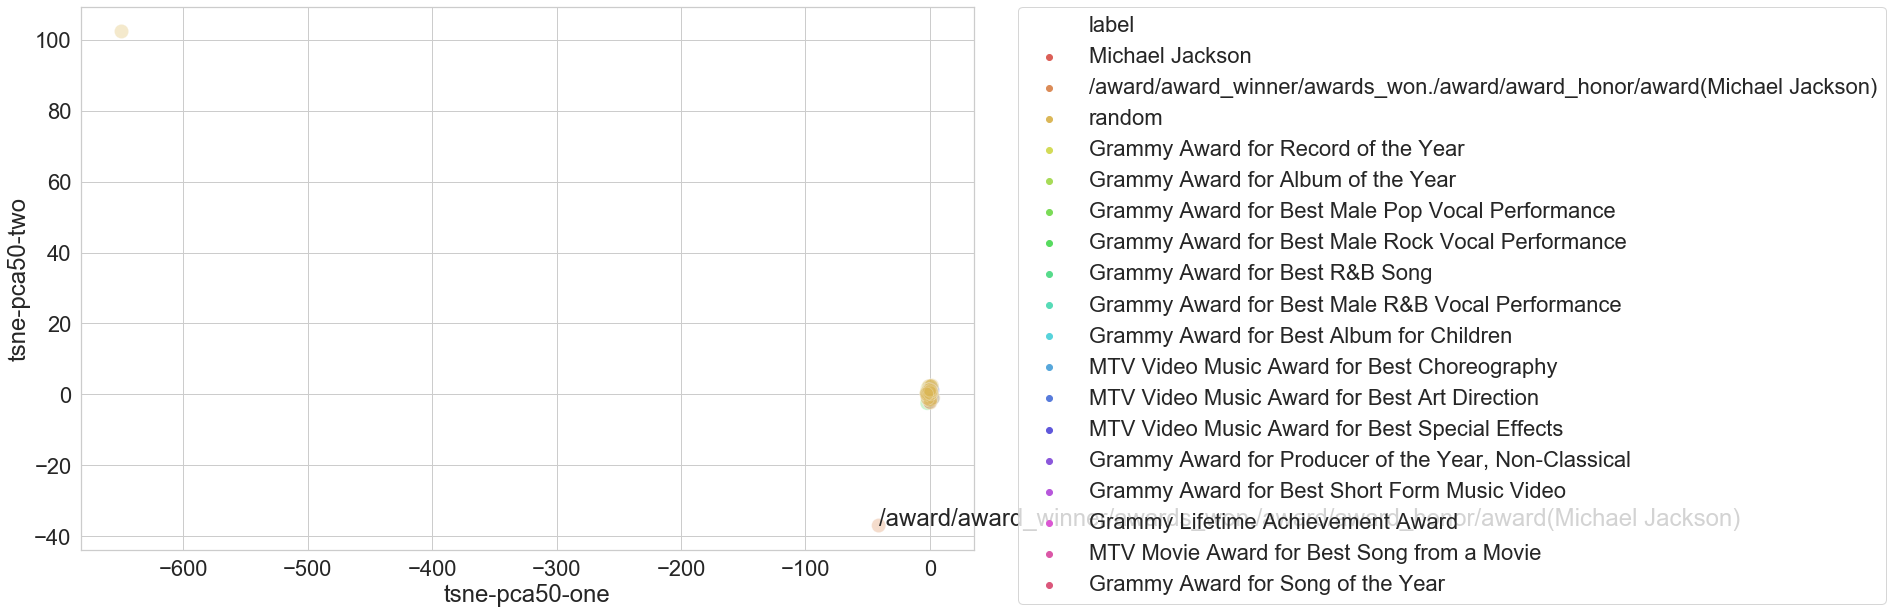
\includegraphics[width=0.7\textwidth, height=0.3\textheight]{t_sne_train_award}
	\captionsetup{justification=centering}
	\caption{FB15k T-SNE: Triples about "Michael Jackson"'s (subject) "awards" (predicate), pre HypER+ training. The legend lists all awards (objects) known to have been won by Michael Jackson. Once again most objects in the KG, regardless of type, are clustered in the same embedding region.}
\end{figure}

\begin{figure}
   	\centering
    	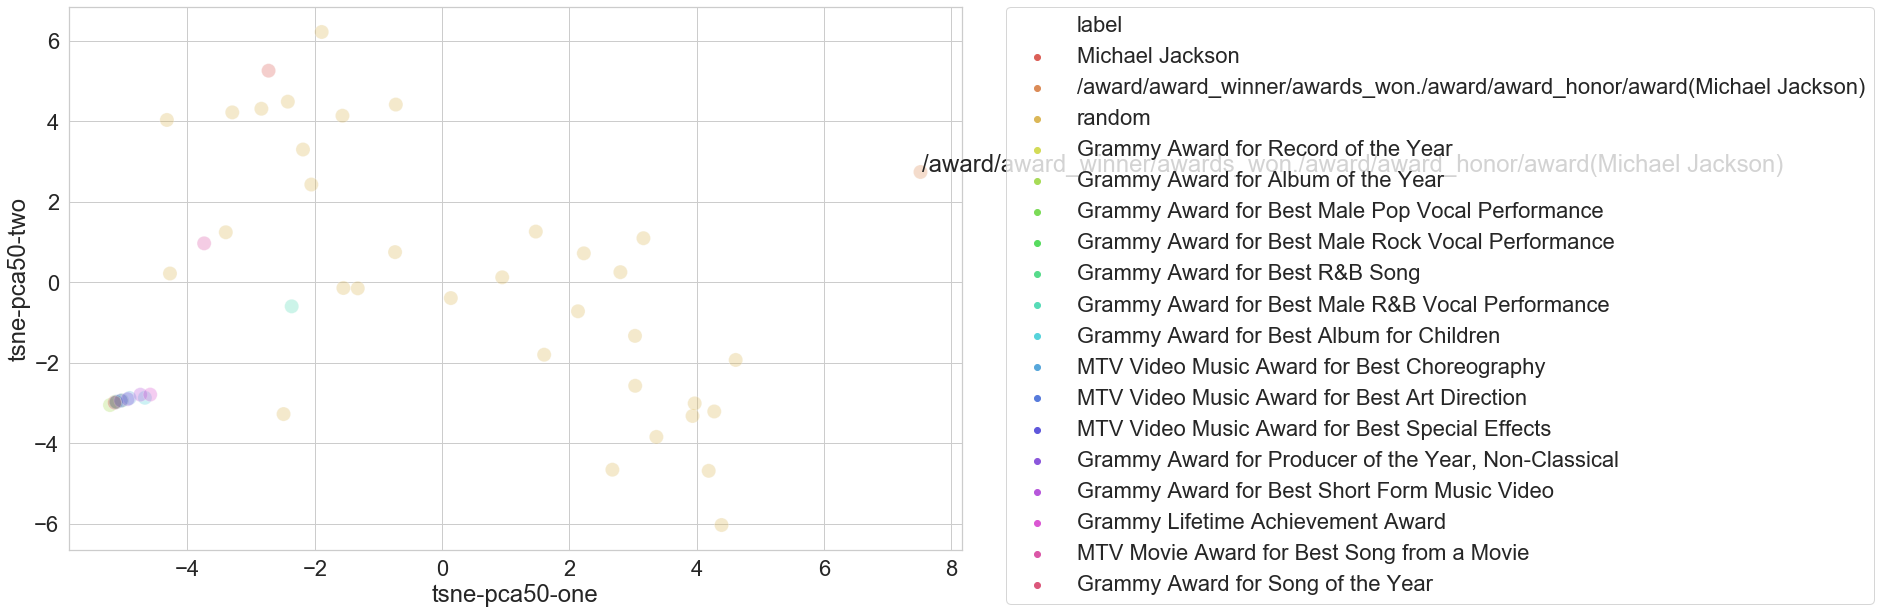
\includegraphics[width=0.7\textwidth, height=0.3\textheight]{t_sne_test_award}
	\captionsetup{justification=centering}
	\caption{FB15k T-SNE: Triples about "Michael Jackson"'s (subject) "awards" (predicate), post HypER+ training. Awards Michael Jackson is known to have won are now somewhat clustered within the same embedding region. This indicates the model has built some conceptual understanding around the objects, and attempts to account for sub-domain differences, as well as conceptual differences between the awards. For example, the "MTV Movie Award for Best Song from a Movie" is located in a region relatively far from all the "Music"-related awards.}
\end{figure}


%********************************** %HypER+ with Pre-Trained Word Embeddings  **************************************

\section{HypER+ with pre-trained word vectors}

\subsection{Datasets} 
For the third and final set of experiments we use the WN18RR and FB15k-237 benchmark datasets.\ WN18RR is a subset of WN18, created by Dettmers et al. \unskip~\citep{dettmers2018convolutional} through removing the inverse relations from WN18. WN18RR contains $ 40, 943 $ entities, $ 11 $ relations and $ 40,943 $ triples. FB15k-237 was created by Toutanova et al. \unskip~\citep{toutanova2015observed}, who noted that the validation and test sets of FB15k and WN18 contain the inverse of many relations present in the training set, making it easy for simple models to do well. FB15k-237 is a subset of FB15k with the inverse relations removed. It contains $ 14, 541 $ entities, $ 237 $ relations and $ 14,541 $ triples. Visualisations of the respective KGs, as well as a sample of RDF triple encoded facts, are presented in Figures 4.26 to 4.29. KG summary statistics are presented in Figures 4.30 to 4.33, and Table 4.6. 

\begin{figure}
   	\centering
    	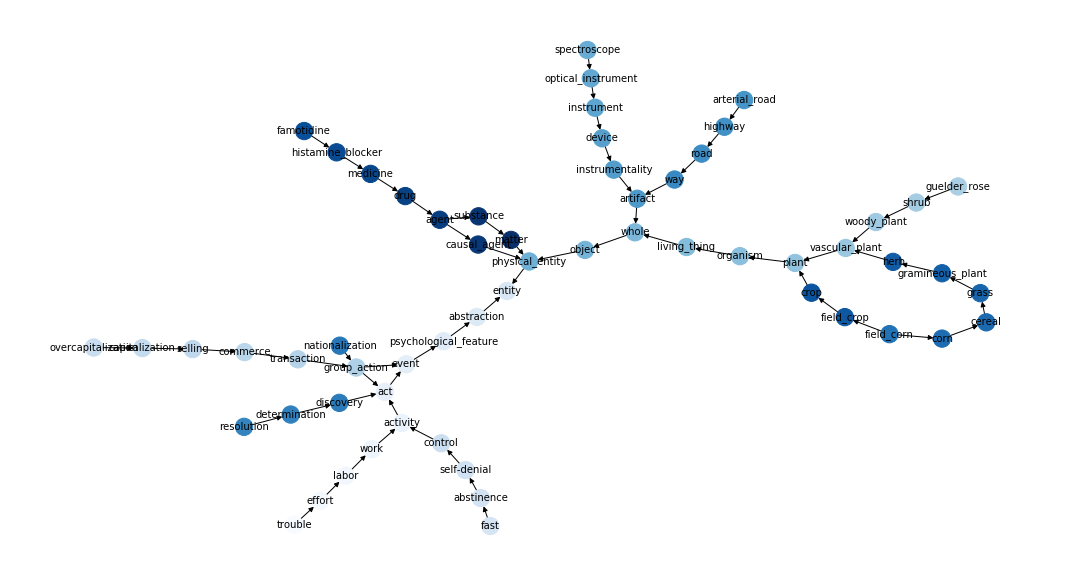
\includegraphics[width=0.9\textwidth, height=0.6\textwidth]{WN18RR_Graph}
	\captionsetup{justification=centering}
	\caption{A subset of WN18RR facts structured as a KG. Entities are nodes, and relations are edges, where facts are encoded as RDF triples.}
\end{figure}

\begin{figure}
   	\centering
    	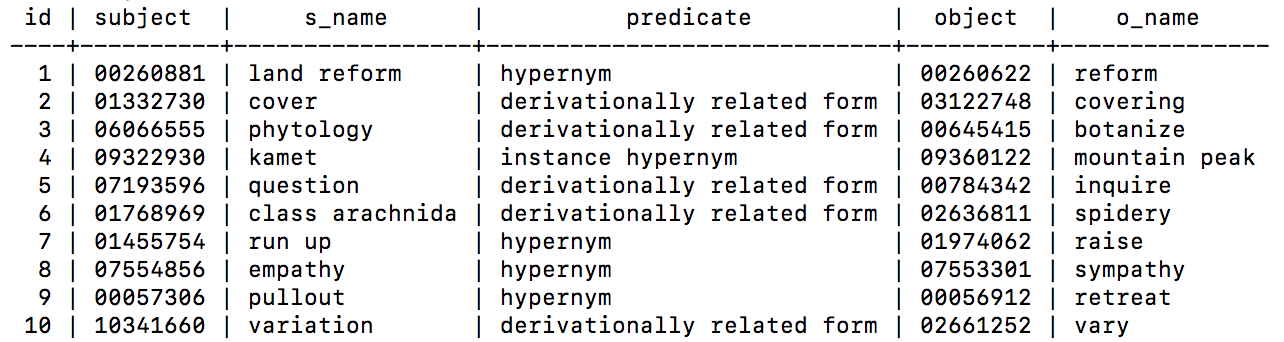
\includegraphics[width=0.9\textwidth, height=0.3\textwidth]{wn18rr_fact_sample}
	\captionsetup{justification=centering}
	\caption{A sample of RDF triples from the WN18RR KG.}
\end{figure}

\begin{figure}
   	\centering
    	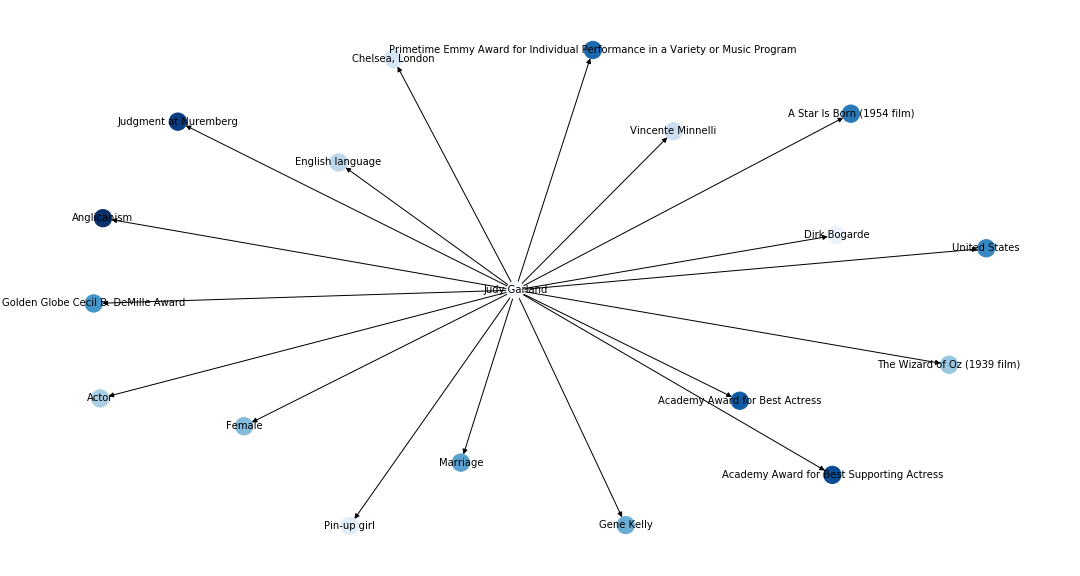
\includegraphics[width=0.9\textwidth, height=0.6\textwidth]{FB15k-237_Graph}
	\captionsetup{justification=centering}
	\caption{A subset of FB15k-237 facts structured as a KG. Entities are nodes, and relations are edges, where facts are encoded as RDF triples.}
\end{figure}

\begin{figure}
   	\centering
    	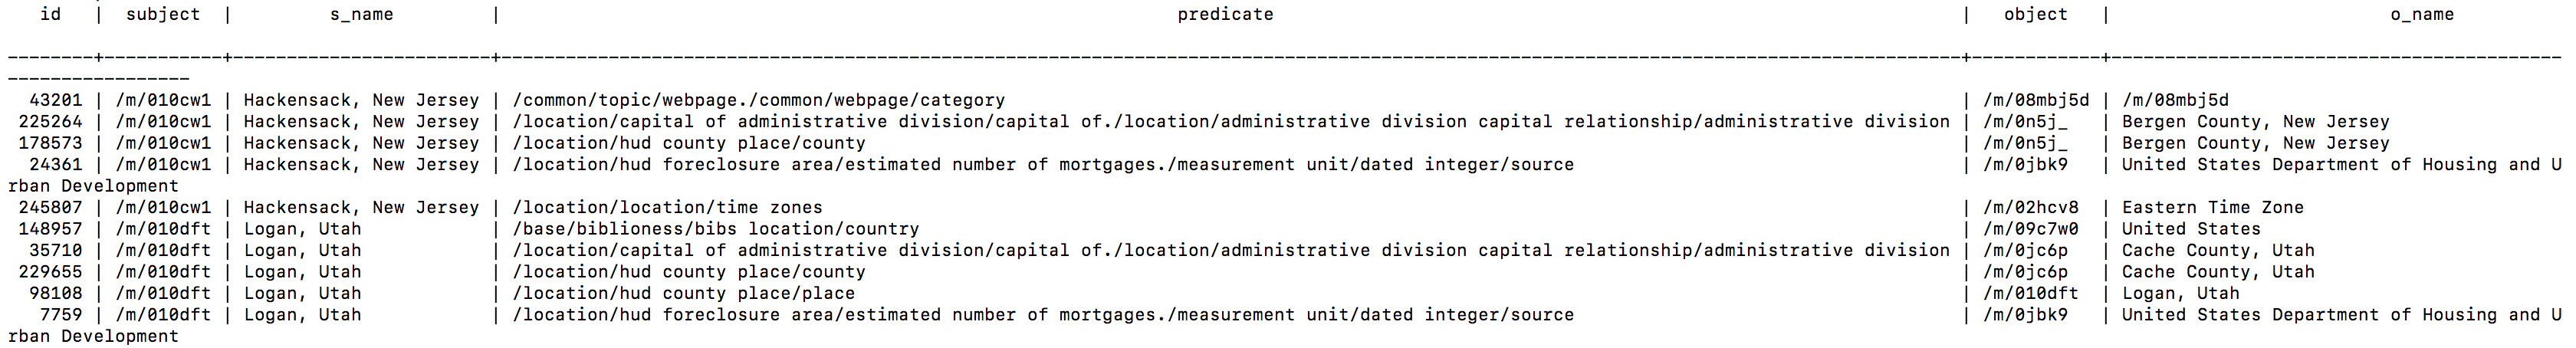
\includegraphics[width=1.0\textwidth, height=0.3\textwidth]{fb15k_237_fact_sample}
	\captionsetup{justification=centering}
	\caption{A sample of RDF triples from the FB15k-237 KG.}
\end{figure}

%********************************** %Subject **************************************

\begin{figure}
	\begin{subfigure}[b]{.5\linewidth}
   		\centering
    		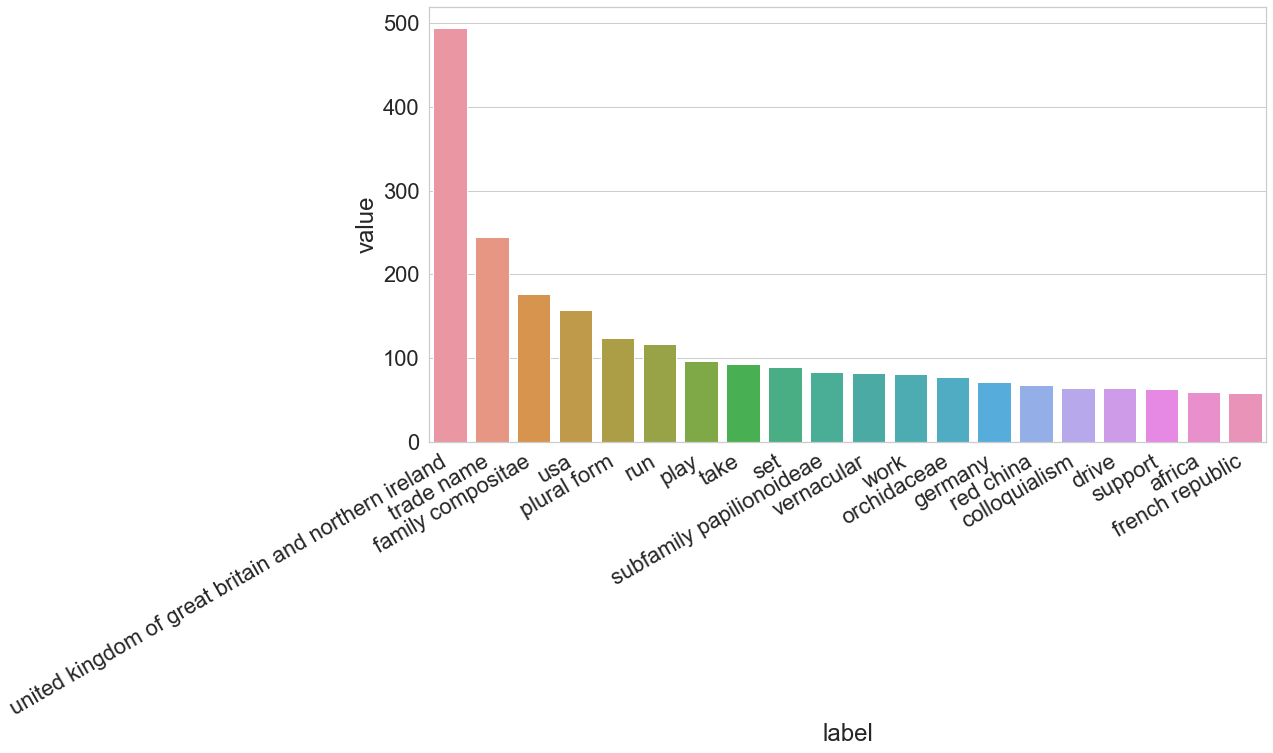
\includegraphics[width=1.0\linewidth, height=0.7\linewidth]{WN18RR_Subject_Counts}
		\captionsetup{justification=centering}
		\caption{WN18RR}
	\end{subfigure}
	\begin{subfigure}[b]{.5\linewidth}
   		\centering
		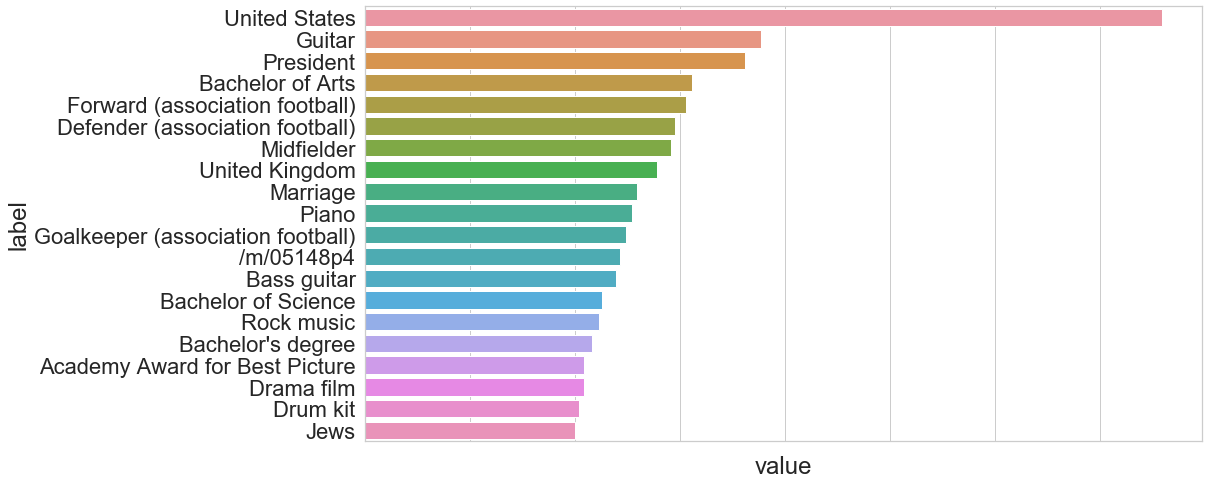
\includegraphics[width=1.0\linewidth, height=0.7\linewidth]{FB15k-237_Subject_Counts}
		\captionsetup{justification=centering}
		\caption{FB15k-237}
	\end{subfigure}
	\captionsetup{justification=centering}
	\caption{Histogram showing the number of times the 20 most frequent subject labels occur in KG facts, in the WN18RR and FB15k-237 link prediction datasets.}
\end{figure}

\bigskip
\bigskip


%********************************** %Predicate **************************************

\begin{figure}
   	\centering
    	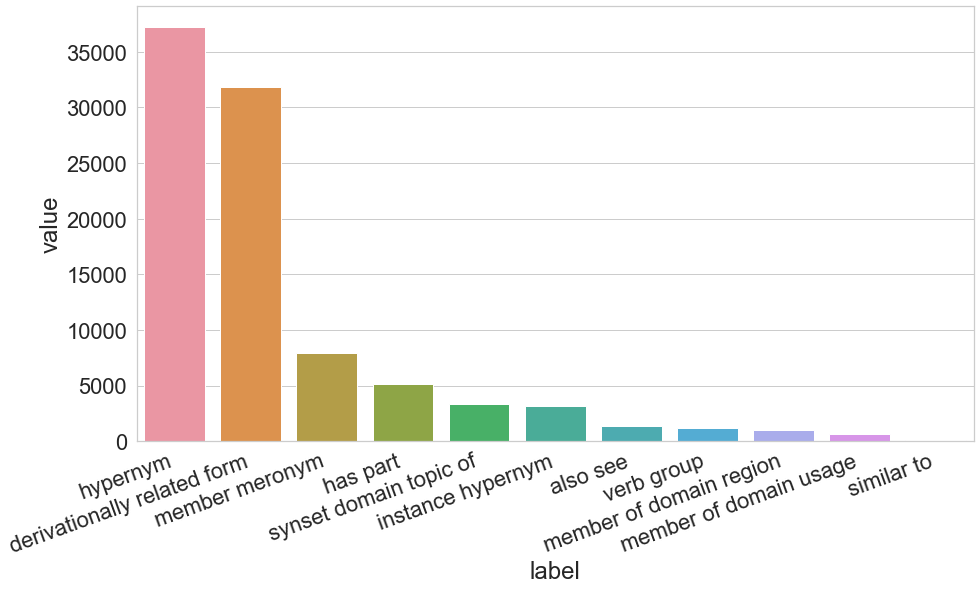
\includegraphics[width=0.7\textwidth, height=0.3\textheight]{WN18RR_Predicate_Counts}
	\captionsetup{justification=centering}
	\caption{Histogram showing the number of times predicate labels occur in KG facts, in the WN18RR link prediction dataset.}
\end{figure}

\begin{figure}
   	\centering
    	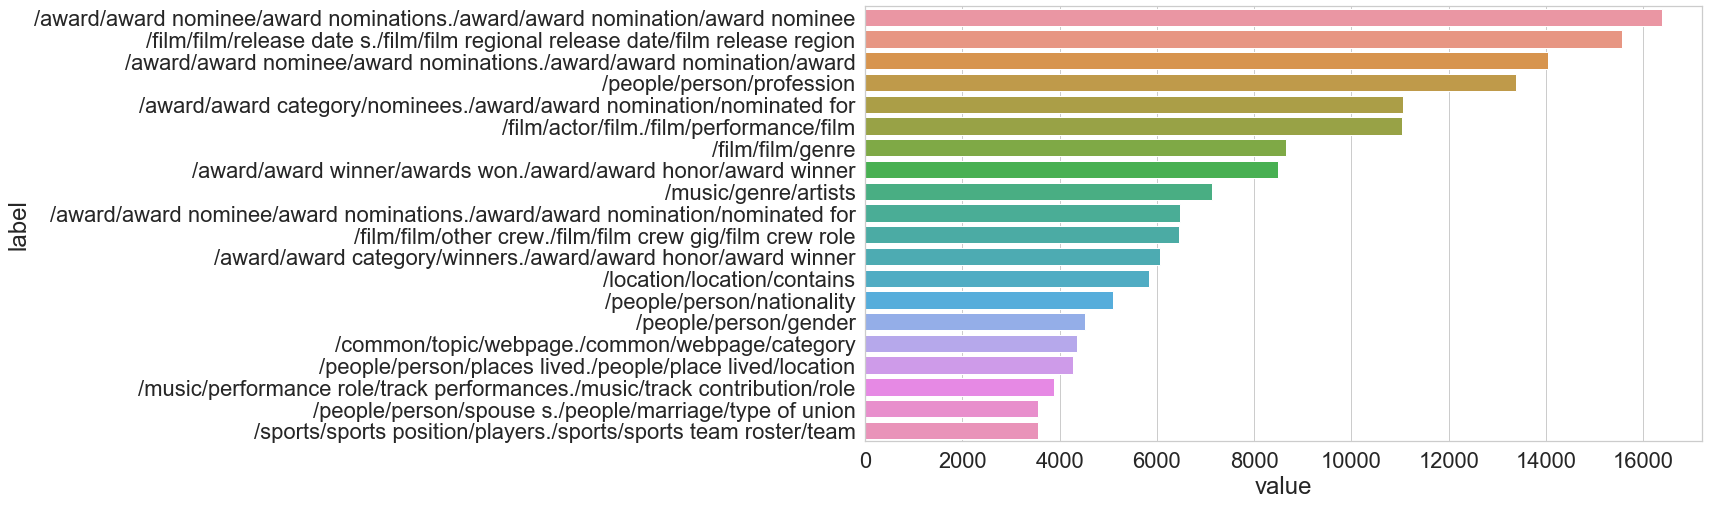
\includegraphics[width=1.0\textwidth, height=0.3\textheight]{FB15k-237_Predicate_Counts}
	\captionsetup{justification=centering}
	\caption{Histogram showing the number of times the 20 most frequent predicate labels occur in KG facts, in the FB15k-237 link prediction dataset.}
\end{figure}


%********************************** %Object **************************************

\begin{figure}
	\begin{subfigure}[b]{.5\linewidth}
   		\centering
    		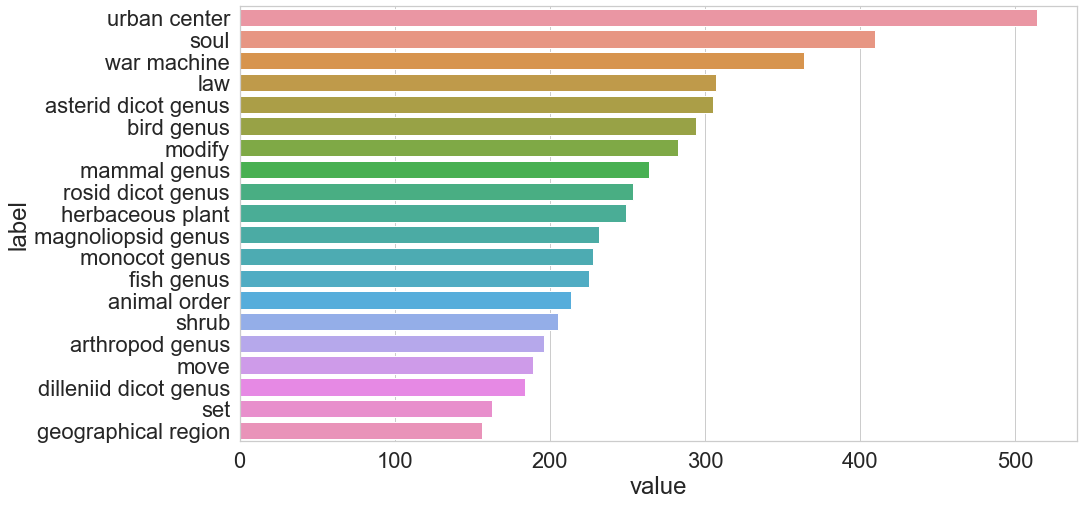
\includegraphics[width=1.0\linewidth, height=0.7\linewidth]{WN18RR_Object_Counts}
		\captionsetup{justification=centering}
		\caption{WN18RR}
	\end{subfigure}
	\begin{subfigure}[b]{.5\linewidth}
   		\centering
		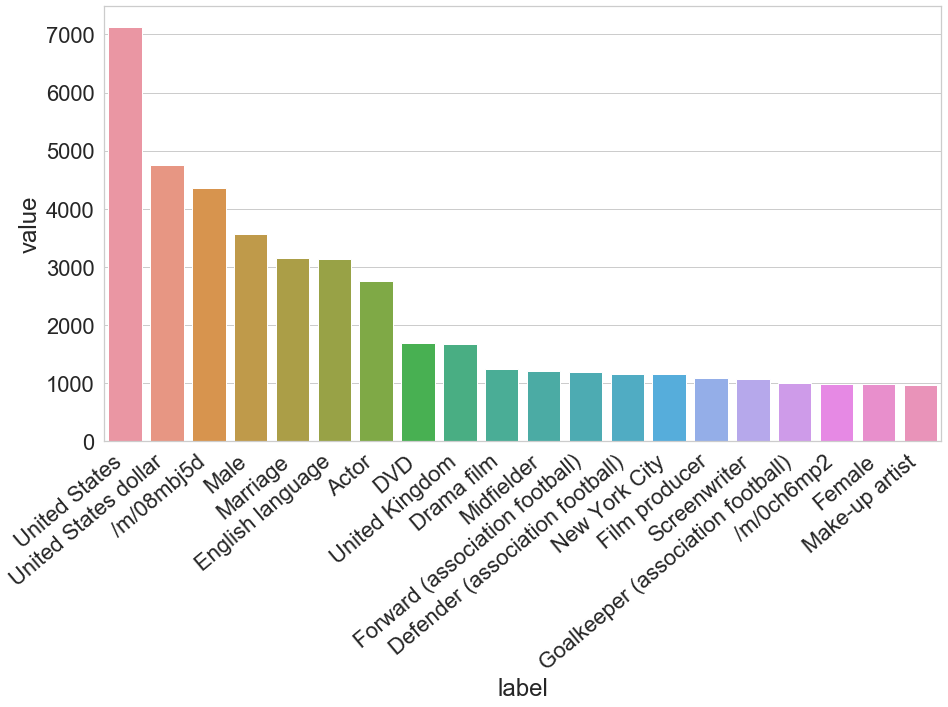
\includegraphics[width=1.0\linewidth, height=0.7\linewidth]{FB15k-237_Object_Counts}
		\captionsetup{justification=centering}
		\caption{FB15k-237}
	\end{subfigure}
	\captionsetup{justification=centering}
	\caption{Histogram showing the number of times the 20 most frequent object labels occur in KG facts, in the WN18RR and FB15k-237 link prediction datasets.}
\end{figure}

\begin{table}[H]
	\begin{center}
	\begin{tabular}{|l|ccc|ccc|}
		\hline
 		& \multicolumn{3}{c|}{\textbf{WN18RR}} & \multicolumn{3}{c|}{\textbf{FB15k-237}} \\
		& subject & predicate & object & subject & predicate & object \\
		\hline 
		Count & 32,349 & 11 & 26,162 & 13,891 & 237 & 13,504 \\
		Max & 494 & 37,221 & 514 & 1,518 & 16,391 & 7,124 \\
		Min & 1 & 86 & 1 & 1 & 45 & 1 \\
		Median & 2 & 3150 & 1 & 16 & 426 & 10 \\
		IQR & 2 & 5434 & 2 & 20 & 819 & 16 \\
		\hline 
	\end{tabular}
	\end{center}
	\captionsetup{justification=centering}
	\caption{Statistics of the WN18RR and FB15k-237 link prediction datasets. We show counts of unique subject, predicate and object labels, as well as the maximum, minimum, median and interquartile range of label occurrences.}
\end{table}

\noindent For WN18RR, it can be seen that predicates are skewed toward the relations "hypernym" and "derivationally related from", with a maximum of $ 37, 221 $ occurring, and an IQR of $ 5434 $ and $ 819 $ respectively. FB15k-237 predicates are skewed toward the film relation. \par

\noindent WN18RR and FB15k-237 subjects are somewhat uniform aside from a small number of high occurring entities, with the median number of occurrences being $ 2 $ and $ 16 $ respectively, and with an IQR of $ 2 $ and $ 20 $ respectively. WN18RR object occurrences are also somewhat uniform, while FB15k-237 object occurrences are skewed, with the "United States" partaking in the highest number of triples. This is in comparison to a median object occurrence of $ 1 $ and $ 10 $, and an IQR of $ 2 $ and $ 16 $ respectively. \par

\noindent The WN18RR dataset is split into a training, validation and test sets of $ 86, 835 \; (93.4 \%) $, $ 3, 034 \; (3.3 \%) $ and $ 3, 134\; (3.4 \%) $ triples respectively.\ The FB15k-237 dataset is split into a training, validation and test sets of $ 272, 115 \; (87.8 \%) $, $ 17, 535 \; (5.7 \%) $ and $ 20, 466 \; (6.6 \%) $ triples respectively.

\subsection{Baseline algorithm}
\textbf{Model summary.} HypER+, introduced in Section 4.2.3, is a model which compensates for covariate shift caused by hypernetworks, by applying batch normalisation to the hypernetwork input layer. The same algorithm as the HypER model is then used to produce a relational score, which is passed through a logistic sigmoid to generate a probability of a potential relationship between pairs of entities.\ HypER+ makes use of Xavier initialised entity and relation embeddings, and is trained using the binary cross-entropy loss. \par


%********************************** %Pre-Trained Word Embeddings **************************************

\subsection{GloVe word vector initialisation}

\textbf{Implementation.} We use the PyTorch framework to develop the HypER+ model with pre-trained embeddings, which is built on top of HypER+.\ Pre-trained GloVe word vectors replace Xavier initialised entity and relational embeddings for model training.\ These embeddings are dynamically adjusted during the training process to generate latent representations specific to the KG. The models in this section were trained on Google Cloud Platform, on an N1 series instance with  8 CPU cores, 30GB RAM, 512GB SSD and an Nvidia Tesla P100 GPU. We train the respective models for $ 500 $ epoch, and evaluate them using the test sets of WN18RR and FB15k-237. \par 

\noindent \textbf{Code to reproduce.} In the interest of reproducibility, all code needed to train and test the models in this section can be found at the following links. \newline
Baseline HypER+: \url{https://github.com/xhosaBoy/HypER-normalised-relations} \newline
HypER+ with GloVe word vectors: \url{https://github.com/xhosaBoy/HypER-pretrained-word-vectors} \par

\subsubsection{Results}
Current standard link prediction metrics (Hit@10, Hit@3, Hit@1, Mean Rank and Mean Reciprocal Rank) are used to first compare the HypER+ model without pre-trained embeddings gainst the HypER+ model with pre-trained embeddings. The results are presented in Figures 4.32 and 4.33, as well as Tables 4.7 and 4.8. Qualitative results are presented in Figure 4.34 and Table 4.9. \par

\noindent HypER+ with pre-trained embeddings gives state-of-the-art (SOTA) performance across both WN18RR and FB15k-237.\ Pre-trained word embeddings have a particularly pronounced impact on the WN18RR Hit@10 and Hit@3 metrics, perhaps due to the smaller number of samples in this KG. They however have limited impact on the Hit@1 metric, where HypER+ without pre-trained embeddings achieves SOTA performance.


%********************************** %Hits@10 **************************************

\begin{figure}
	\begin{subfigure}[b]{.5\linewidth}
   		\centering
    		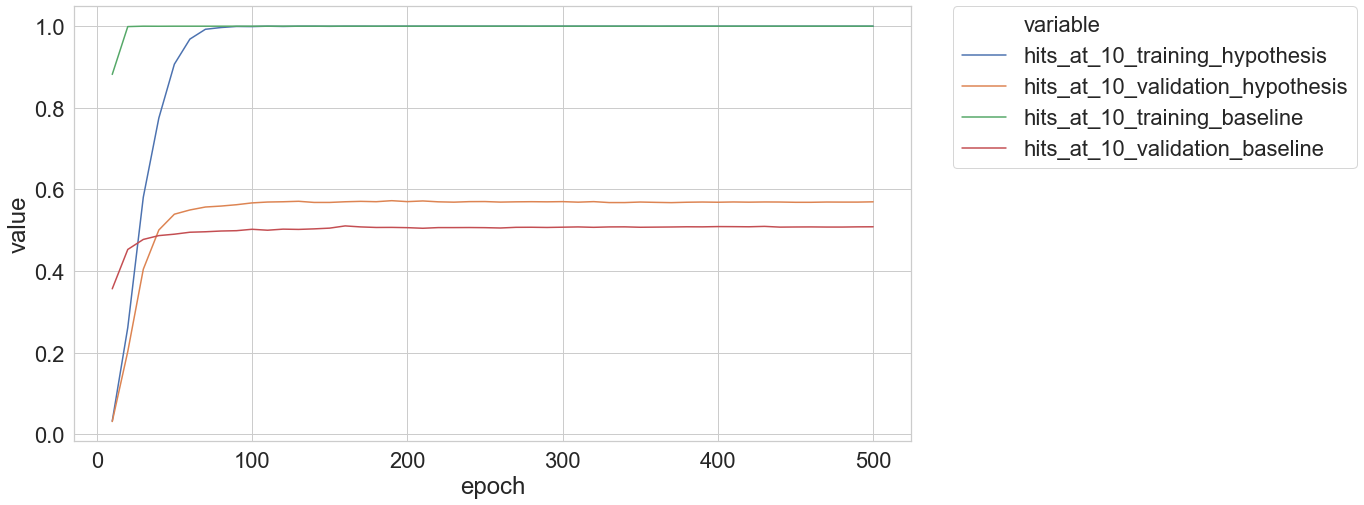
\includegraphics[width=1.0\linewidth, height=0.5\linewidth]{WN18RR_hits_at_10_Results_ptwv}
		\captionsetup{justification=centering}
		\caption{WN18RR: HypER+ vs \\ HypER+ with pre-trained embeddings}
	\end{subfigure}
	\begin{subfigure}[b]{.5\linewidth}
   		\centering
		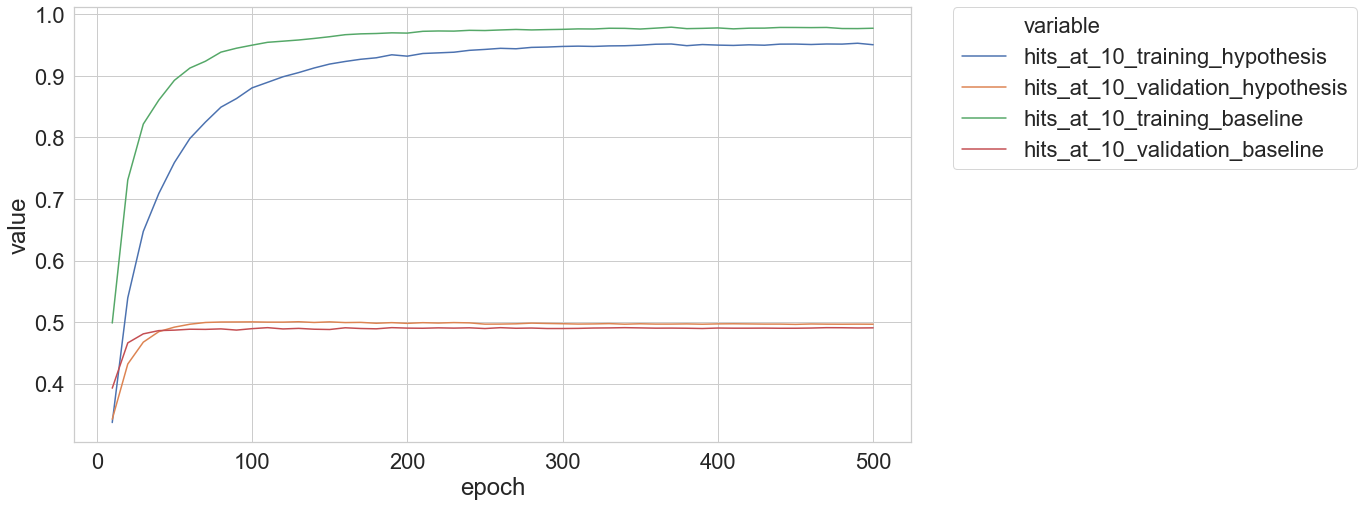
\includegraphics[width=1.0\linewidth, height=0.5\linewidth]{FB15k-237_hits_at_10_Results_ptwv}
		\captionsetup{justification=centering}
		\caption{FB15k-237: HypER+ vs \\ HypER+ with pre-trained embeddings}
	\end{subfigure}
	\captionsetup{justification=centering}
	\caption{Hit@10 vs training epoch. The hypothesis significantly outperforms the baseline on the WN18RR KG. The hypothesis only marginally outperforms the baseline on the FB15k-237 KG. This suggests pre-trained embeddings have more of an impact on smaller KGs, where relations are likely to be more sparse, making it harder to build entity and relation conceptual understanding.}
\end{figure}


%********************************** %Mean rank **************************************

\begin{figure}
	\begin{subfigure}[b]{.5\linewidth}
   		\centering
    		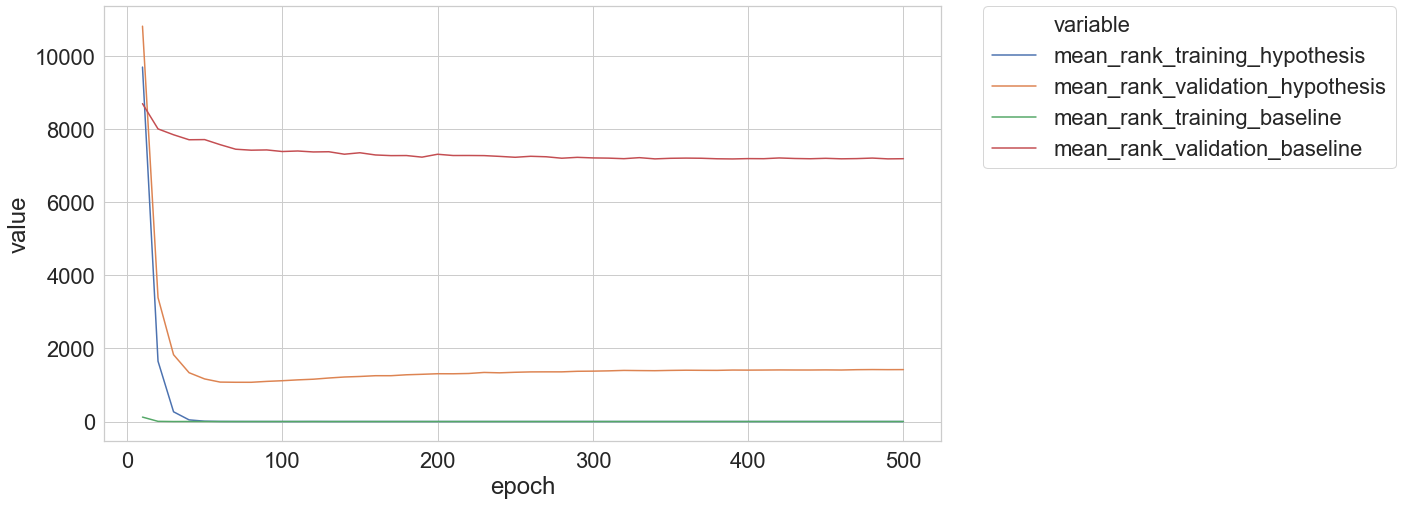
\includegraphics[width=1.0\linewidth, height=0.6\linewidth]{WN18RR_mean_rank_Results_ptwv}
		\captionsetup{justification=centering}
		\caption{WN18RR: HypER+ vs \\ HypER+ with pre-trained embeddings}
	\end{subfigure}
	\begin{subfigure}[b]{.5\linewidth}
   		\centering
		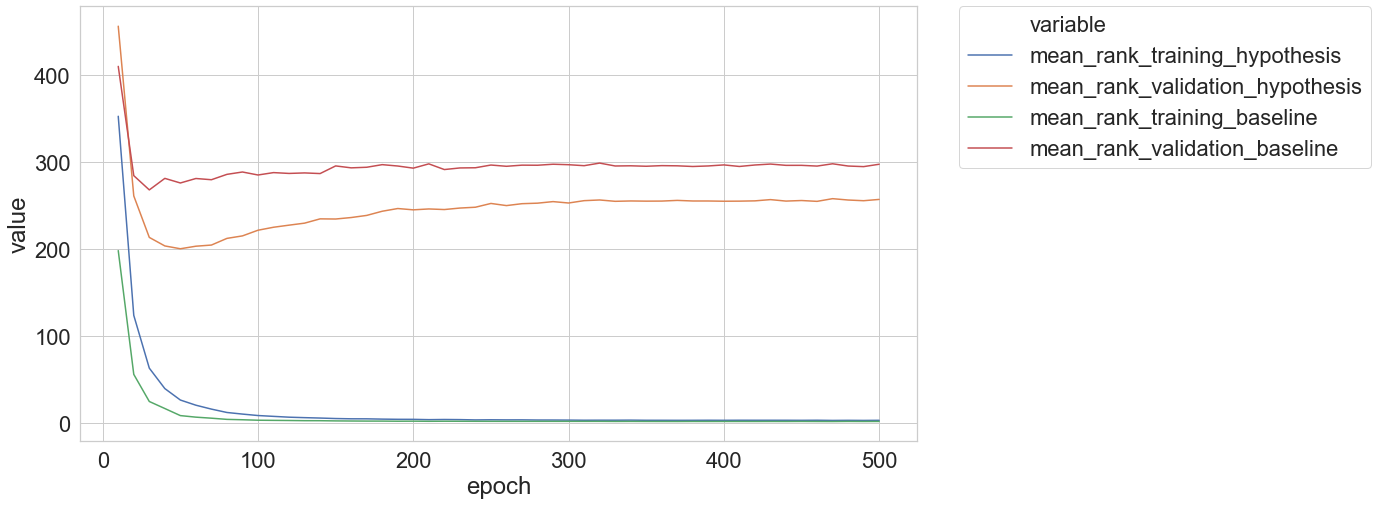
\includegraphics[width=1.0\linewidth, height=0.6\linewidth]{FB15k-237_mean_rank_Results_ptwv}
		\captionsetup{justification=centering}
		\caption{FB15k-237: HypER+ vs \\ HypER+ with pre-trained embeddings}
	\end{subfigure}
	\captionsetup{justification=centering, name={Figure}}
	\caption{Mean Rank vs training epoch. There is a stark difference in performance between the hypothesis and baseline on the WN18RR KG. Pre-trained embeddings are very effective at providing semantic information that can be used to produce good predictions for smaller, less complex KGs. The difference is less pronounced on the FB15k-237 KG, however is still significant.}
\end{figure}


%********************************** %Test results **************************************

\begin{table}
		\centering
		\begin{tabular}{lllllllllll}
  			\textbf{Model} & \textbf{H@10} & \textbf{H@3} & \textbf{H@1} & \textbf{MR} & \textbf{MRR} \\
  			\hline
  			DistMult \unskip~\citep{yang2014embedding} & .490 & .440 & .390 & 5110 & .430 \\
  			ComplEx \unskip~\citep{trouillon2016complex} & .510 & .460 & .410 & 5261 & .440 \\
  			Neural LP \unskip~\citep{yang2017differentiable} & - & - & - & - & - \\
			ConvE \unskip~\citep{dettmers2018convolutional} & .520 & .440 & .400 & 4187 & .430 \\
			HypER \unskip~\citep{balazevic2019hypernetwork} & .522 & .477 & .436 & 5798 & .465 \\
			HypER+ (ours) & .519 & .479 & \textbf{.438} & 7061 & .466 \\
  			\hline
  			HypER+ with pre-trained embeddings (ours) & \textbf{.578} & \textbf{.493} & .435 & \textbf{1063} & \textbf{.480} \\
			&
		\end{tabular}
		\captionsetup{justification=centering}
		\caption{Relation prediction test results on WN18RR. HypER+ with pre-trained word embeddings significantly outperforms both the HypER as well as HypER+ models. HypER+ outperforms HypER+ with pre-trained embeddings on the Hit@1 metric, consistent with the expectation of diminished impact of pre-trained embeddings at high levels of accuracy constraints. It should be noted that there is a difference of $ 0.3 \% $ between all three models (HypER, HypER+ and HypER+ with pre-trained word embeddings), suggesting almost identical performance. The largest differences in performance occur at Hit@10 and Mean Rank, bearing the effectiveness of pre-trained embeddings at compensating for sparsity, however also highlighting how their significance diminishes at higher levels of accuracy. }
\end{table}

\begin{table}
		\centering
		\begin{tabular}{lllllllllll}
  			\textbf{Model} & \textbf{H@10} & \textbf{H@3} & \textbf{H@1} & \textbf{MR} & \textbf{MRR} \\
  			\hline
  			DistMult \unskip~\citep{yang2014embedding} & .419 & .263 & .155 & 254 & .241 \\
  			ComplEx \unskip~\citep{trouillon2016complex} & .428 & .275 & .158 & 339 & .247 \\
  			Neural LP  \unskip~\citep{yang2017differentiable} & .408 & - & - & - & .250 \\
			ConvE \unskip~\citep{dettmers2018convolutional} & .501 & .356 & .237 & 244 & .325 \\
			HypER \unskip~\citep{balazevic2019hypernetwork} & .520 & .376 & .252 & 250 & .341 \\
			HypER+ (ours) & .516 & .368 & .245 & 268 & .335 \\
  			\hline
  			HypER+ with pre-trained embeddings (ours) & \textbf{.525} & \textbf{.379} & \textbf{.255} & \textbf{196} & \textbf{.345} \\
			&
		\end{tabular}
		\captionsetup{justification=centering}
		\caption{Relation prediction test results on FB15k-237. The HypER+ model with pre-trained embeddings achieves state-of-the-art performance across all metrics. Covariate shift seems to not be playing as meaningful a role, and pre-trained embeddings are providing a more meaningful contribution, as suggested by the HypER+ model's inferior performance to the HypER model. Strangely, this is inconsistent with training and validation set results, where HypER+ consistently outperforms HypER on FB15k-237. The fact that we use the quoted HypER test results, as opposed to reimplemented and verified test results, may explain this inconsistency. This inconsistency aside, pre-trained embeddings remain effective at improving relation prediction performance on the FB15k-237 KG.}
\end{table}


%********************************** %Test Result Decomposition **************************************

\begin{figure} [H]
   	\centering
    	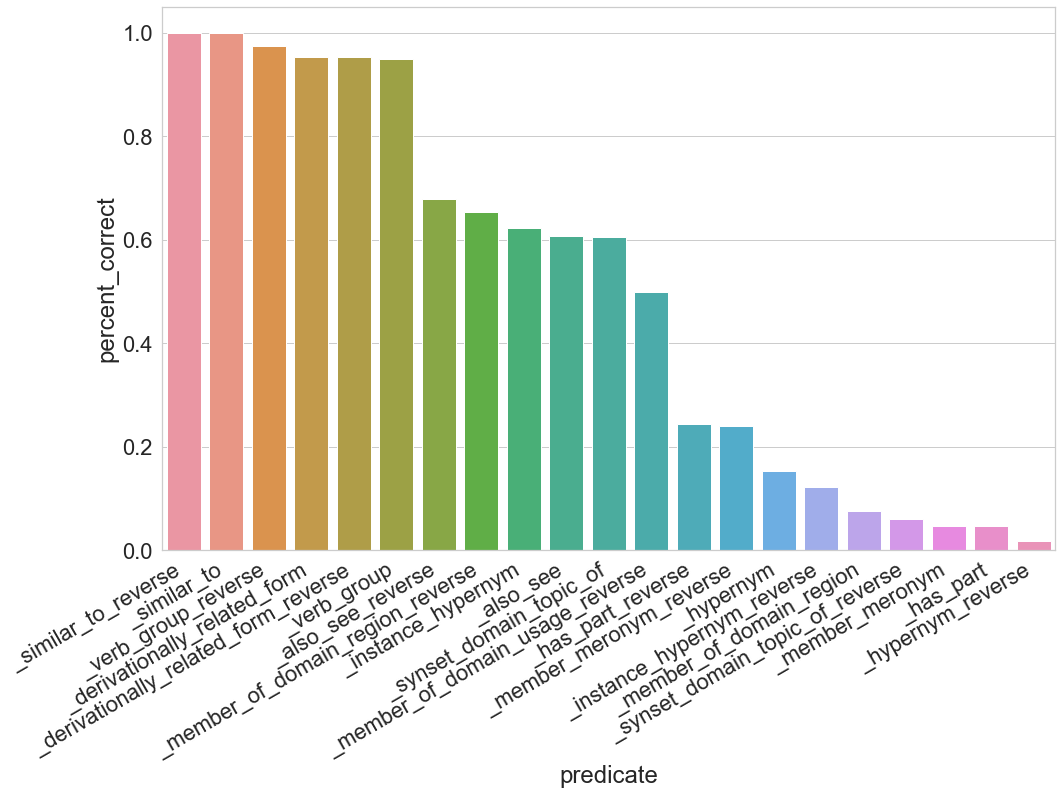
\includegraphics[width=0.7\textwidth, height=0.3\textheight]{WN18RR_relational_performance_results}
	\captionsetup{justification=centering}
	\caption{WN18RR Hit@1 predicate performance of the HypER+ model with pre-trained embeddings. The model performs well with synonym relation types, but performs poorly with compositional and hierarchical relations. This may be due to the inherent similarity and analogy in concepts, whereas compositions and hierarchies can be defined by strict rules. Perhaps, more simply, it could be due to the number of test set samples for each relation, where higher numbers increase the prediction error rate.}
\end{figure}

\bigskip
\bigskip
\bigskip
\bigskip

\begin{table}[H]
	\centering
	\resizebox{1.0\columnwidth}{!}{
	\begin{tabular}{lllllllllll}
  		\textbf{Subject} & \textbf{Predicate} & \textbf{Object Target} & \textbf{Object Prediction} \\
  		\hline
  		usa & has part & colorado & missouri river \\
  		spain & has part & cadiz & jerez de la frontera \\
  		kilobyte & has part & computer memory unit & word \\
		electromagnetic spectrum & has part & actinic ray & radio spectrum \\
		systema respiratorium & has part & respiratory tract & respiratory organ \\
		respiratory organ & has part & nsa & defense advanced research projects agency \\
		africa & has part & nigeria & senegal \\
  		antigen & has part & substance & epitope \\
		amphitheatre & has part & theatre & tiered seat \\
		indian ocean & has part & mauritius & antarctic ocean \\
		&
	\end{tabular}
	}
	\captionsetup{justification=centering}
	\caption{Qualitative Hit@1 test results on WN18RR. The table presents a set of questions posed to the HypER+ with pre-trained embeddings model. "Object Target" is the expected answer, and "Object Prediction" is the answer given by the model. The model demonstrates basic conceptual understanding, never making mistakes that would be considered obvious by humans. We would expect reasonable knowledge discovery utility from the model, when used jointly with information retrieval for open-domain question answering \unskip~\citep{chen2017reading}. }
\end{table}


%********************************** %Chapter Summary  **************************************

\section{Summary}

\textbf{NTN with optimised training algorithm.}\ We attempted to improve the NTN model by applying training algorithm optimisations including early stopping, the Adam optimiser and hyperparameter random search. The results indicate that there are potential performance gains to be realised simply through using training algorithm techniques known to improve performance. In this instance we see an accuracy gain of 6.2\% across the WordNet and Freebase datasets. \par

\noindent \textbf{HypER+.}\ We compensated for possible covariate shift introduced by hypernetworks.\ The latent representation distribution drift of relations is pronounced enough that we are able to improve the Hit@1 accuracy of the original HypER model on average by 2.7\%, across the WN18 and FB15k KGs.\ We note graph modelling may be a worthwhile paradigm to explore for link prediction, given R-GCN's SOTA performance for Hit@10 accuracy on the WN18 KG. We also note the greater influence of relational normalisation on prediction performance for larger and more complex KGs. \par

\noindent \textbf{HypER+ with pre-trained word vectors.}\ Finally we extended HypER+ to make use of pre-trained GloVe word vectors.\ The semantic information inherent in these embeddings significantly improves relation prediction performance on sparse relational data. Their influence is somewhat reduced at higher levels of accuracy, where KG domain alignment becomes more important. Pre-trained word vectors also offer less utility for large and complex KGs, however still contribute an improvement to prediction. The combination of relation normalisation, and entity and relation embedding initialisation using pre-trained word vectors, both addresses the problems of data sparsity, as well as produces higher quality relational latent representations for large and complex datasets. As a result, HypER+ with pre-trained word vectors achieves SOTA performance on almost all standard link prediction benchmark metrics, across the challenging WN18RR and FB15k-237 KGs. 
